\documentclass[nonblindrev,copyedit]{informs1}

\usepackage{natbib}
\bibpunct[, ]{(}{)}{,}{a}{}{,}
\def\bibfont{\small}
\def\bibsep{1pt plus .3ex}
\def\bibhang{24pt}
\def\newblock{\ }
\def\BIBand{and}

\usepackage{amsmath,amssymb,mathtools}
\usepackage{mathpazo}
\usepackage{graphicx}
\usepackage[justification=centering]{caption}
\usepackage{subcaption}
\usepackage{hyperref}

\TheoremsNumberedThrough

\begin{document}
\RUNAUTHOR{Jiang et al. (2026)}
\RUNTITLE{Dynamic Competition with C2C}

\TITLE{Dynamic Competition in Online Retailing: Implications of Customer-to-Customer Interactions}

\ARTICLEAUTHORS{
\AUTHOR{Zheyu Jiang}
\AFF{School of Management and Engineering, Nanjing University, \EMAIL{zheyujiang@nju.edu.cn}}
\AUTHOR{Xin Geng}
\AFF{Miami Herbert Business School, University of Miami, \EMAIL{xgeng@bus.miami.edu}}
\AUTHOR{Nan Yang}
\AFF{Miami Herbert Business School, University of Miami, \EMAIL{nyang@bus.miami.edu}}
\AUTHOR{Renyu Zhang}
\AFF{CUHK Business School, The Chinese University of Hong Kong, \EMAIL{philipzhang@cuhk.edu.hk}}
}
\ABSTRACT{
\emph{Problem Definition:}
Online retailing has increasingly become socially embedded, with customers frequently engaging in customer-to-customer (C2C) interactions such as reviews, social media posts, and recommendations, which significantly shape their purchase decisions. In a competitive context, we distinguish two types of C2C interactions: \emph{Within-brand} interactions direct incremental future demand toward the originating retailer, whereas \emph{cross-brand} interactions generate a shared market benefiting competitors. This paper aims to investigate how different types of C2C interactions influence online retailers' dynamic competition.
\emph{Methodology/Results:}
We formulate a two-period duopoly game between newsvendor-type online retailers with asymmetric costs. Stockout-based substitution occurs within periods, and C2C interactions regulate market evolution across periods. We derive equilibrium outcomes and obtain three major findings.
First, under cross-brand C2C interactions, the higher-cost retailer tends to stock less initially compared to the within-brand scenario, strategically leveraging the lower-cost retailer's larger stockpile and benefiting from market expansion at reduced inventory cost, a form of free-riding behavior.
Second, equilibrium profit comparisons across scenarios can yield non-intuitive results. Specifically, the lower-cost (advantaged) retailer might achieve higher profits under cross-brand interactions, as shared market growth softens competition. Conversely, the higher-cost (disadvantaged) retailer can benefit more under within-brand interactions, which intensify competition but allow it to capture benefits from the cultivated customer base.
Third, when retailers have pricing flexibility, equilibrium prices exhibit contrasting trends for sufficiently strong C2C interactions. Under within-brand C2C, prices increase over time as each retailer’s current sales build seller-specific future demand. In contrast, under cross-brand C2C, prices decline across periods as retailers aggressively compete to secure larger shares of the jointly expanded market.
\emph{Managerial Implications:}
Our results provide valuable managerial insights: Online retailers must carefully identify the dominant form of C2C interactions in their markets.
Moreover, effective inventory and pricing strategies must align with the prevailing type of social interactions in dynamic competitive environments.
}

\maketitle

\section{Introduction}

\footnote{The verification repo, which includes all the code that reproduces the numerical results of this paper, is available on GitHub: \url{https://github.com/rphilipzhang/dynamic-competition-c2c}.}Ever since online retailing was born, it has been constantly redefined by business-model and technological innovations. In recent years, with the rapid growth of social media platforms (e.g., Facebook, YouTube, and X), online retailing has evolved into a more interactive and socially embedded mode, where consumer behavior is increasingly shaped by interpersonal influences and shared experiences. One notable phenomenon is the prevalence of customer-to-customer (C2C) interactions, such as product reviews, outfit posts, unboxing videos, and other user-generated content across social platforms. These interactions, both verbal and visual, can significantly impact consumer demand and product visibility across brands and categories.

Practical examples abound in the fashion sector. Consider two online retailers, such as Amazon Fashion and Shein, both selling seasonal clothing. In the fall, they run promotional campaigns that include live video shopping events. After customers receive their purchases, many begin to share styling tips and outfit hauls through TikTok and Instagram. These posts, often in informal and brand-agnostic formats, not only influence the visibility of one retailer but also stimulate demand for the fashion category at large. When winter arrives, a new group of customers who were exposed to this content may enter the market, with some drawn to the brand they saw and others simply attracted to the category. This social contagion process expands the market for both retailers, though not always equally, depending on the nature of the interactions. Such behavior is now widespread across many sectors of online retailing and is especially amplified during short but intense selling periods, such as those surrounding e-commerce holidays like Singles Day and Cyber Monday.

To better understand this dynamic, we distinguish between two types of C2C interactions. When communications by a retailer's existing customers---such as reviews, recommendations, or product-specific social content---direct incremental demand toward the same brand, we refer to this as a \textit{within-brand} C2C interaction. For example, an unsolicited customer TikTok featuring Aerie's Crossover Leggings triggered extensive follow-up content and product searches, followed by repeated sellouts \citep{businessinsider2021}. Similarly, customer videos featuring UNIQLO's Round Mini Shoulder Bag went viral and were followed by a marked increase in the product's sales \citep{guardian2023uniqlo}. These examples illustrate how customer communications can stimulate subsequent demand for the focal brand. Empirical studies likewise document social learning and product trial in online fashion and identify customer-driven trend effects in fashion transaction data \citep[see, e.g.,][]{lee2013,baardman2023}. By contrast, when C2C communications generate broader interest in a product category rather than directing demand toward a particular brand, we refer to this as a \textit{cross-brand} C2C interaction. For example, Miu Miu's ballet flats became Lyst's most-searched flat shoe during the fall of 2022, while searches for ``ballet flats'' more broadly increased by 400\% \citep{fashionista2022miumiu}. Alaïa's fishnet Mary Janes and The Row's mesh slippers have similarly been credited with popularizing a mesh-flat trend subsequently adopted by competing brands \citep{forbes2024mesh}. The Adidas--Puma terrace-shoe episode provides another example: growing social-media attention to retro terrace styles concurrently increased demand opportunities for competing brands \citep{reuters2023terrace,reuters2024puma}.
Moreover, empirical evidence indicates that sales-generated future demand need not be confined to the originating brand. In the soft-drink market, \cite{cola2020} find that category-related eWOM can benefit competing brands; in the video-game market, \cite{haviv2020} document positive intertemporal demand spillovers across competing products. More broadly, \cite{libai2009} distinguish within-brand and cross-brand communications in competitive growth. Together, these prior studies motivate examining whether sales-generated future demand benefits only the originating seller or is shared with competitors. Our contribution is to analyze the operational incentives and equilibrium consequences of this distinction.

Whether within-brand or cross-brand, C2C interactions create a dependence between current decisions and future demand for retailers, because current sales, which are determined by pricing and stocking decisions, affect the future market size and structure. Importantly, recognizing the nature of these interactions, retailers may respond differently in managing the trade-off between current profitability and future growth, potentially leading to contrasting equilibrium strategies and managerial insights. Therefore, the central objective of this paper is to understand how the structures of C2C interactions shape dynamic competition among online retailers. To that end, we develop a two-period duopoly model in which two newsvendor-type retailers with asymmetric costs compete in each period over price and inventory (via stockout-based substitution), and the market evolves across periods due to C2C interactions. As a key feature, our model explicitly incorporates both within-brand and cross-brand interactions and studies their respective implications for competitive dynamics. Then, we address the following research questions. Treating prices as exogenously given, how do the system parameters such as social contagion strength and competition intensity jointly determine the retailers' strategic stocking decisions under each type of C2C interaction? How does each retailer’s profit change and compare under different types of C2C interactions? When prices are endogenously and dynamically decided, how do the retailers' pricing strategies affect earlier results?

To start, we examine the retailers’ stocking strategies under exogenously given retail prices. We find that the low-cost retailer orders more aggressively when competition intensifies, as this expands its future market and improves profitability. The high-cost retailer, in contrast, exhibits more nuanced behavior: Under within-brand C2C interactions (Scenario S), it orders a large quantity regardless of competition; under cross-brand C2C interactions (Scenario N), it strategically reduces its order quantity as competition intensifies. This behavior reflects a form of operational free-riding. By ordering less, the high-cost retailer allows unmet demand to spill over to its low-cost rival, which in turn helps grow the shared market under Scenario N. Such a result highlights an important managerial insight: A high-cost firm may benefit from deliberately relying on its rival’s sales to stimulate market growth, rather than investing in costly inventory itself.

Next, we compare the retailers' equilibrium profits under the two forms of C2C interactions. While it may be intuitive to expect that the low-cost retailer performs better under the more competitive within-brand interactions, and the high-cost retailer prefers the collaborative nature of cross-brand interactions, our results show that this intuition does not always hold. Depending on key parameters such as market share split, cost asymmetry, social interaction strength, and competition intensity, each retailer’s profit can be higher or lower in either scenario.
For example, when the social interactions are strong, the change in the price difference between the two retailers across periods can serve as the main driver of the profit comparison. If the price difference stays the same, other parameters start to drive the comparison results:
When the cost advantage and competition level are substantial, the low-cost retailer may actually earn more under Scenario N, because the joint market expansion outweighs the costs of intensified competition. Conversely, when the high-cost retailer is not at a significant disadvantage, it may benefit more from Scenario S, where it can appropriate the future demand benefit generated by its own realized sales. Since the two C2C interaction structures give rise to a blend of competitive and cooperative forces, the results contribute to the understanding of the notion of coopetition \citep{coop1996,coop2001}. From a strategic management standpoint, we offer key managerial insights into how firms can navigate the tension between rivalry and collaboration, and recognize when it is in their best interest to pursue a more balanced coopetitive relationship.

Finally, we extend the model to a two-period price-inventory game where both retailers endogenously choose their prices and order quantities. This richer framework reveals new strategic dynamics in how pricing interacts with the two types of C2C interactions. We find that under Scenario S, equilibrium prices increase over time; i.e., retailers initially lower prices to grow their own customer base, and later exploit this advantage. In contrast, under Scenario N, prices decline over time as firms compete for a greater share of the jointly expanded market. Notably, the downward pricing trend under Scenario N reflects a strategic effort to capture a larger share of the common market, particularly in the second period when the value created by demand expansion in the first period is realized. These pricing dynamics, together with our earlier findings, suggest that the strategic use of price as a competitive lever depends critically on the structure of customers' social interactions. Moreover, our numerical analysis shows that the qualitative comparisons of profits across scenarios largely persist even with pricing flexibility, provided that the strength of social interactions is not excessively large.
From a marketing perspective, our findings suggest that firms operating in socially connected environments must account for how peer influence propagates across brands versus within brands, and adapt pricing strategies accordingly.

\section{Literature Review}\label{sec:lit}

Our work belongs to the literature on retail operations at large \citep[see a comprehensive review by][]{ckm2020}. Specifically, four streams of studies are closely related to our paper.

The first stream examines the relationship between C2C interactions and generated demand. Existing empirical research supports a dynamic process in which purchases create opportunities for customer communication, which in turn can affect later demand. In particular, \cite{goh2013,adamopoulos2018}, and \cite{vana2021} document how user-generated content, word-of-mouth (WOM) exposure, and individual reviews affect subsequent purchasing behavior; the meta-analysis of \cite{babicrosario2016} establishes positive average relationships between eWOM and sales; \cite{fu2023} show the operational value of social-media information for fashion-demand forecasting; through randomized experiments, \cite{burtch2018} find that combining financial incentives and social-norm information generates the greatest overall contribution of online reviews. Together, these studies corroborate the directional linkage of sales, C2C interactions, and future demand in our model. Unlike this literature, our study embeds this linkage in a strategic two-period price-inventory competition model.

Following the above stream of literature, a second stream further studies the different mechanisms through which C2C communications affect demand. The distinction between within-brand and cross-brand C2C interactions in our model draws directly on the taxonomy proposed by \cite{libai2009}, whose pioneering work provides a theoretical foundation for analyzing social contagion in competitive settings. Since then, a growing stream of research has extended this framework to study various managerial issues under different modeling approaches and contexts \citep[see, e.g.,][]{ksv12, godes17, geng22}. Some studies examine settings in which C2C communications primarily affect demand for the focal seller or brand, corresponding to the within-brand interaction in our model. For example, \cite{lee2013} document social learning and product trial in online fashion, \cite{baardman2023} uncover C2C trend effects in fashion transaction data, and \cite{duan2008} and \cite{zhou2015} study the dynamic feedback between sales, WOM, and subsequent sales. Other studies investigate how customer communications generate social spillovers across competing firms or related products, corresponding to our cross-brand interaction. In particular, \cite{cola2020} find that Pepsi-related eWOM, classified as ``category news'', is positively associated with the sales of both Pepsi and Coke, \cite{shi2023} identify both cannibalization and market-expansion effects in fashion, \cite{cho2024} and \cite{kwark2021} show that reviews of competing or related products affect focal demand, and \cite{haviv2020} provide causal evidence of positive intertemporal demand spillovers across rival products. Our paper contributes to this stream by incorporating these interaction mechanisms into a dynamic pricing-inventory game, where competitive outcomes are endogenously determined.

The third literature stream is on inventory competition and stockout-based substitution. \cite{lm1997} establish the classical competitive-newsvendor model framework, and \cite{netessine2003} build upon it to study centralized and competitive inventory systems with demand substitution. More recently, \cite{bansal2022} extend this literature to multiple competitors and multistage spillovers of unmet demand. Empirical studies also present complementary grounding for the theoretical model: \cite{lee2016} estimate stockout-based substitution and demonstrate its operational importance, \cite{li2023} show with large-scale fashion data that unmet demand is partially redirected to available alternatives, and \cite{ergin2022} document demand shifts across neighboring fast-fashion stores following stockouts. In our model, the assumption that stockout-based demand substitution occurs within each period is rooted directly in this literature. Furthermore, our paper contributes to this literature by examining how such substitution interacts with the market-growth mechanism driven by C2C interactions.

The fourth relevant literature stream is on dynamic inventory competition \citep[see, e.g.,][]{hp2000,lsw2007,nagarajan2008,nagarajan2009,olsen2008,olsen2014} and price-setting newsvendors \citep[see, e.g.,][]{pd1999,za2008,sa2011}. These problems have long been studied in the inventory literature under various settings, and the extant papers provide us with useful methodological tools for analyzing the dynamic inventory and pricing decisions. However, our paper has a different scope and research agenda; more importantly, we differ from the prior works because the demand evolution in our paper is shaped by C2C interactions. Thus, we contribute to the literature by incorporating an important marketing consideration into a dynamic setting. Being closely tied to inventory decisions on the one hand and regulating market diffusion on the other, C2C interactions play a pivotal role in online retailing that merits careful consideration.

\section{General Model Framework}\label{model:framework}

We study a two-period duopoly competition in which two online retailers sell substitutable perishable products and the market evolves across periods through C2C interactions. In each period, the retailers compete in price and inventory, while stockout-based substitution may redirect unmet demand from one retailer to the other. We first describe the firms, then present the aggregate demand dynamics in the order in which they arise, and finally conclude the section by formulating the retailers' dynamic optimization problems.

\subsection{Firms}

Consider two online retailers, A and B, selling substitutable perishable products in two consecutive sales seasons (periods). For example, Amazon Fashion and Shein may both offer fall collections (e.g., plaid jackets and Halloween-themed apparel) and winter collections (e.g., fur jackets and holiday-themed clothes). In period $t$, retailer $i$ ($i=A,B$) sets its price $p_{i,t}$ and then decides its stocking level $y_{i,t}$. The two retailers are asymmetric in unit ordering cost, $c_i$. Without loss of generality, retailer A has a lower unit ordering cost than retailer B, i.e., $c_A<c_B$.

Products are perishable within our two-period setting. Any leftovers at the end of a period are salvaged through other channels, and we normalize the salvage value to zero. Likewise, unmet demand does not carry over across selling seasons. This assumption is particularly natural for seasonal fashion products whose product categories and purchase occasions change across successive seasons.

\subsection{Demand and Market Dynamics}

The demand process consists of three components that arise sequentially: (i) seed demand is generated and split between the retailers; (ii) prior realized sales generate market growth through C2C interactions; and (iii) after inventory availability is resolved, stockouts may induce substitution between the retailers.

\subsubsection{Seed Demand and Demand Split.}

In every period $t$, there is a seed demand $X_t$ representing the common underlying market for the two retailers. The sequence $\{X_t\}$ is i.i.d. with distribution $F(\cdot)$ and density $f(\cdot)$. In the seasonal-fashion example, this seed demand captures consumers who enter the market because of recurring seasonal purchase needs or social norms, independently of the C2C interactions that occurred in the previous period.

The seed demand is initially split between the two retailers. Let $\alpha_{i,t}$ denote retailer $i$'s share, where $\alpha_{A,t}+\alpha_{B,t}=1$. Following the deterministic demand-splitting approach in \cite{lm1997}, but allowing the split to depend on prices, we assume
\[
    \alpha_{i,t}
    =\alpha_{i,t}(p_{i,t},p_{j,t})
    =\frac{1}{2}+\beta(p_{j,t}-p_{i,t}),
    \qquad i,j=A,B;\ i\neq j,
\]
where $\beta>0$ captures the sensitivity of the aggregate demand share to price differences. Thus, retailer $i$ receives $\alpha_{i,t}X_t$ units of the seed demand before C2C-induced demand is added.

\subsubsection{Market Growth through C2C Interactions.}

Prior customers may subsequently generate reviews, recommendations, styling posts, try-on hauls, and other customer-generated content. Such C2C communications can affect later product trial and therefore be informative for future fashion demand \citep[see supporting evidence in, e.g.,][]{lee2013,baardman2023}. We therefore use realized sales in the previous period as the aggregate customer base from which subsequent C2C-induced demand may arise.

Let $Z_{i,t}$ denote retailer $i$'s incremental C2C-induced demand. Retailer $i$'s demand before any current-period stockout occurs is then
\begin{equation}
M_{i,t}=\alpha_{i,t}X_t+Z_{i,t}.
\label{general}
\end{equation}
We refer to $M_{i,t}$ as retailer $i$'s \emph{pre-stockout demand}. The form of $Z_{i,t}$ depends on whether the C2C interaction is primarily within-brand or cross-brand.

\paragraph{Within-Brand C2C Interactions (Scenario S).}
Under within-brand C2C, communication generated by a retailer's prior customers directs incremental demand toward that retailer. This can occur when customer-generated content contains seller- or product-specific information that reduces uncertainty, facilitates product trial, or otherwise increases interest in the focal seller's offering. As mentioned in Section 1, the viral Aerie leggings and UNIQLO shoulder-bag episodes illustrate this mechanism \citep{businessinsider2021,guardian2023uniqlo}; moreover, empirical studies document social learning, product trial, and customer-driven trend effects in online fashion \citep[see, e.g.,][]{lee2013,baardman2023}.

We model this case as $Z_{i,t}^S=\gamma R_{i,t-1}^S$, where $\gamma>0$ captures the strength of C2C-induced market growth and $R_{i,t-1}^S$ is retailer $i$'s realized sales in the previous period. Hence,
\begin{equation}
M_{i,t}^S=\alpha_{i,t}X_t+\gamma R_{i,t-1}^S .
\label{sne}
\end{equation}
Thus, under Scenario S, the additional demand generated by retailer $i$'s previous customers enters retailer $i$'s pre-stockout demand.

\paragraph{Cross-Brand C2C Interactions (Scenario N).}
Customer communication may instead increase interest in a broader product category, style, functionality, or use occasion rather than direct the additional demand toward the originating retailer. Real-world stories about Miu Miu ballet-flat, mesh-flat, and Adidas--Puma terrace-shoe illustrate how attention surrounding particular products can broaden into category-level interest that competing brands may capture \citep{fashionista2022miumiu,forbes2024mesh,reuters2023terrace, reuters2024puma}. Empirical studies likewise document such spillovers across competing products \citep[e.g.,][]{cola2020,haviv2020,shi2023}. We refer to this case as cross-brand C2C, or Scenario N.

Let $R_{t-1}^N=R_{A,t-1}^N+R_{B,t-1}^N$ denote total realized sales in the previous period. Under Scenario N, these sales generate an incremental common market $\gamma R_{t-1}^N$, which is subsequently split between the two retailers according to the same rule, characterized by $\alpha_{i,t}$, as for the seed demand of that period. Therefore, $Z_{i,t}^N=\alpha_{i,t}\gamma R_{t-1}^N$, and
\begin{equation}
M_{i,t}^N=\alpha_{i,t}\left(X_t+\gamma R_{t-1}^N\right).
\label{nne}
\end{equation}
The distinction between Scenarios S and N is therefore where the C2C-induced incremental demand enters the competitive market. Under within-brand C2C, it is attributed to the originating retailer, whereas under cross-brand C2C, it first expands the common market and is then divided between the retailers.

\subsubsection{Stockout-Based Substitution.}

The first two components determine each retailer's pre-stockout demand $M_{i,t}$. Stockout-based substitution occurs subsequently, after current-period inventory availability is resolved. Importantly, under within-brand C2C, the fact that the C2C-induced demand is initially directed toward the same retailer does not imply that these customers are unaware of competing alternatives after inventory availability is known. Once a stockout is observed, search, recommendations, or other availability information may direct customers to the competing retailer and enable substitution. If retailer $j$ stocks out, a fraction $\theta\in[0,1]$ of its unmet pre-stockout demand is redirected to retailer $i$. Therefore, retailer $i$'s effective demand is
\[
D_{i,t}=M_{i,t}+\theta\left(M_{j,t}-y_{j,t}\right)^+, \qquad i,j=A,B;\ i\neq j.
\]
A larger $\theta$ represents a greater degree of stockout-based substitution and hence more intense inventory competition. This formulation follows the classical competitive inventory model and is consistent with empirical evidence that stockouts can redirect part of unmet demand toward available alternatives \citep[see, e.g.,][]{lee2016,li2023,ergin2022}.
Finally, retailer $i$'s realized sales and period profit are $R_{i,t}=\min\{D_{i,t},y_{i,t}\}$ and $\pi_{i,t}=p_{i,t}R_{i,t}-c_i y_{i,t}$, respectively.

\subsubsection{Remarks.}

The three components above describe the aggregate market dynamics used in our analysis: seed demand is first split between the retailers, prior realized sales then generate C2C-induced demand, and stockout-based substitution finally reallocates part of unmet demand after inventory availability is resolved. Our aggregate demand system is not derived from a formal consumer-level micro-foundation. The empirical evidence and prior literature motivate these component mechanisms, but do not jointly derive the complete demand system. We therefore use this reduced-form framework to obtain tractable insights into how different types of C2C interactions affect dynamic inventory competition and pricing. Developing an integrated micro-foundation model that jointly captures these mechanisms is an important direction for future research.

\subsection{Problem Formulation}\label{sec:form}

Together, these model elements define a two-period competitive newsvendor problem formulated as a two-player Nash game with complete information. Because the underlying mechanism of C2C interactions becomes operative after one transition between selling seasons, a two-period model is sufficient to isolate its strategic effect while preserving analytical tractability.

The sequence of events in period $t$ is as follows. (1) The retailers observe the previous-period realized sales $(R_{A,t-1},R_{B,t-1})$; for $t=1$, we set $R_{i,0}=0$. (2) The retailers choose prices $p_{i,t}$ and then stocking levels $y_{i,t}$, with each decision made simultaneously across retailers. (3) Seed demand $X_t$ is realized and split according to $\alpha_{i,t}$; when $t=2$, C2C-induced demand generated by previous realized sales is added according to Scenario S or Scenario N, yielding pre-stockout demand $M_{i,t}$. (4) Inventory availability is resolved and stockout-based substitution determines effective demand $D_{i,t}$; realized sales $R_{i,t}$ and profit $\pi_{i,t}$ then follow.

The objective of retailer $i$ is to maximize its total discounted profit across the two periods. As such, retailer $i$ solves
\[
 (\mathcal{P}) \qquad   \max_{p_{i,1},y_{i,1}; p_{i,2},y_{i,2}} \mathbb{E}_{X_1,X_2} \left[ \left( p_{i,1}R_{i,1}-c_iy_{i,1} \right) +\rho\left( p_{i,2}R_{i,2}-c_iy_{i,2} \right) \right] ,
\]
subject to
\[
R_{i,t}=\min\{D_{i,t}, y_{i,t}\},  D_{i,t}=M_{i,t}+\theta (M_{j,t}-y_{j,t})^+,  \mbox{ and } M_{i,t} = \alpha_{i,t} X_t + Z_{i,t}; \quad t=1, 2.
\]
The parameter $0<\rho\leq 1$ is the discount factor. The equilibrium concept adopted is feedback Nash equilibrium. We treat the sales $R_{i,t}$ as state variables in each period, and solve for the prices $p_{i,t}$ and the order quantities $y_{i,t}$ via backward induction.

This two-period model highlights the complexities online retailers face in pricing and inventory management when different types of C2C interactions have significant influences on demand.
However, such price-inventory competition in multiple periods is analytically difficult to solve. Hence, in this paper, we consider two models. First, we assume that the prices in both periods are fixed and study the Exogenous Price Model in Section \ref{sec:main}. Then, in Section \ref{sec:pricing}, we investigate the retailers' pricing decisions in the Endogenous Price Model and derive relevant insights into the impact of pricing flexibility. Lastly, we will set the discount factor $\rho=1$ and assume a uniform distribution for the seed demand for the rest of the paper; that is, let $X_t\sim U[\mu-\sigma,\mu+\sigma]$ for $t=1,2$ ($\mu > \sigma$). Note that we have obtained the equilibrium of the Exogenous Price Model with any $\rho\in(0,1]$ and a general seed demand distribution with interval support and a strictly positive density on the interior of that interval (see the proofs in Appendix A.1). Moreover, we have numerically tested that all our results remain qualitatively the same with other distributions.

\section{Exogenous Price Model}\label{sec:main}

In this section, we assume that retail prices in each period, $p_{i,t}$ ($i=A,B;t=1,2$), are predetermined and fixed. Such an exogenous price model may be suitable considering the practical constraints in the digital selling environment. Livestreaming campaigns, promotional commitments, platform policies, and the seasonal nature of fashion and holiday-themed apparel may discourage short-term price adjustments. Moreover, competitive environments often lead to price convergence at the start of the season, leaving inventory as the primary decision variable for retailers. In the following, we scrutinize the two-period inventory competition between the two retailers; i.e., in period $t$, after the retailers observe the previous sales volumes, they only decide their stocking levels $y_{i,t}$. We first derive the equilibrium of the competition in different scenarios and then present our main findings regarding the equilibrium comparisons between scenarios. To preserve the structural properties of the objective functions, we make a mild technical assumption\footnote{This assumption is made only to obtain structured results in this section; the model can still be solved without it (see Online Appendix). Moreover, we will drop the assumption in the next section for the Endogenous Price Model. } that $p_{B,t}\geq p_{A,t} \geq \frac{c_A}{c_B} p_{B,t}$ for $t=1,2$. Since $c_A<c_B$, it is intuitive that retailer A can set a lower price due to its cost efficiency; our assumption simply requires that the price advantage is not too large.

\subsection{Equilibrium Analysis}\label{model:equil}

\subsubsection{Benchmark Scenario: No C2C Interactions.}
In the benchmark scenario, the market growth across the two periods disappears, and the model is reduced to repeated static games. We directly apply the results from \cite{lm1997} here.
\begin{lemma}
\label{lem:model0}
Suppose there is no C2C interaction. A unique Nash equilibrium exists: $y^{0}_{A,t} = (\alpha_{A,t} + \theta \alpha_{B,t}) \zeta_{A,t}^0 - \theta \alpha_{B,t} \zeta_{B,t}^0$ and $y^{0}_{B,t} = \alpha_{B,t} \zeta_{B,t}^0$, where $\zeta_{i,t}^0= F^{-1}(1 - \frac{c_i}{p_{i,t}})$ ($i = A, B; t= 1, 2$).
\end{lemma}

All proofs in this paper are delegated to Online Appendix A. Note that $\zeta_{i,t}^0$ is exactly the classic newsvendor's critical $z$-score for retailer $i$, and $\zeta_{A,t}^0>\zeta_{B,t}^0$ because $c_A < c_B$. Recall that $F(\cdot)$ is the cdf of the seed demand distribution; hence, for uniform distribution $X_t\sim U[\mu-\sigma,\mu+\sigma]$, $F^{-1}(x)=2\sigma\cdot x+(\mu-\sigma)$. From Lemma \ref{lem:model0}, we have $y^{0}_{A,t} > y^{0}_{B,t}$ for all $\theta$ (see Lemma \ref{lem:oneside}). Thus, the more cost-efficient retailer A always maintains a higher stocking level; retailer B, on the other hand, is in a disadvantageous position in the duopoly relationship due to the cost asymmetry.

\subsubsection{Scenario S.}
Next, we include within-brand C2C in our analysis. This type of interaction among customers is brand specific, and the market dynamic equation is given by \eqref{sne}. In this scenario, it is each retailer's individual past sales that determines the expansion of its own market, so they take advantage of the C2C interactions independently.
\begin{lemma}
\label{lem:models}
Suppose the C2C interactions are within-brand. A unique Nash equilibrium exists: In the first period, $y^{S}_{A,1} = (\alpha_{A,1} + \theta \alpha_{B,1}) \zeta_{A,1}^S - \theta \alpha_{B,1} \zeta_{B,1}^S$ and $y^{S}_{B,1} = \alpha_{B,1} \zeta_{B,1}^S$, where $\zeta^S_{i,1} = F^{-1}\left( 1 - \frac{c_i}{p_{i,1} + \gamma (p_{i,2}-c_i)}\right)$; in the second period, given the two retailers' sales, $R_{A,1}^S$ and $R_{B,1}^S$, $y^{S}_{A,2} = y_{A,2}^0 + \gamma R_{A,1}^S$ and $y^{S}_{B,2} = y_{B,2}^0 +  \gamma R_{B,1}^S$. Moreover, the retailers' equilibrium sales and profits are specified in the appendix.
\end{lemma}

In Scenario S, the retailers' first-period order quantity has the same form as in the benchmark, but with different critical $z$-scores. Moreover, we have $\zeta_{A,1}^S > \zeta_{B,1}^S$ due to the cost asymmetry $c_A < c_B$; as a result, $y^{S}_{A,1} > y^{S}_{B,1}$. For the second-period order quantity $y_{i,2}^S$, it must first satisfy the C2C-induced demand $\gamma R_{i,1}^S$ (contingent on the previous sales), and the rest is the same as the benchmark scenario, due to the end-of-horizon effect. Furthermore, note that the within-brand C2C has effectively raised the underage cost for the retailers in the first period, because stockout means not only losing current customers, but also potential future customers, to the rival. Hence, retailers would order more in the first period compared to the benchmark case (see details in the proof).

\subsubsection{Scenario N.}
Now, we turn to the case where customers engage in cross-brand interactions, which are non-specific in brand names. In Scenario N, the market expansion characterized by \eqref{nne} depends on the retailers’ joint realized sales. The resulting incremental market is shared in the sense that it is subsequently allocated between the retailers according to the market-share rule.
\begin{lemma}
\label{lem:modeln}
Suppose the C2C interactions are cross-brand. A unique Nash equilibrium exists: In the first period, $y^{N}_{A,1} = (\alpha_{A,1} + \theta \alpha_{B,1}) \zeta_{A,1}^N - \theta \alpha_{B,1} \zeta_{B,1}^N$ and $y^{N}_{B,1} = \alpha_{B,1} \zeta_{B,1}^N$, where
\[
\zeta^N_{A,1} = F^{-1} \bigg( 1- \frac{c_A}{p_{A,1} + \alpha_{A,2} \gamma (p_{A,2} -c_A)} \bigg)\text{ and }
        \zeta^N_{B,1}= F^{-1} \bigg( 1- \frac{c_B - \alpha_{B,2} \gamma \theta (p_{B,2} -c_B)  \frac{c_A}{p_{A,1} + \alpha_{A,2} \gamma (p_{A,2}-c_A)}}{p_{B,1} + \alpha_{B,2} \gamma (1-\theta)(p_{B,2} -c_B)} \bigg);
\]
in the second period, given the two retailers' total sales $R_1^N=R_{A,1}^N+R_{B,1}^N$, $y^{N}_{A,2} = y_{A,2}^0 + \alpha_{A,2} \gamma R_{1}^N$ and $y^{N}_{B,2} = y_{B,2}^0 + \alpha_{B,2} \gamma R_{1}^N$. Moreover, the retailers' equilibrium sales and profits are specified in the appendix.
\end{lemma}

Since retailers' first-period sales affect each other's second-period customer acquisition, their order quantities are intertwined, as shown in Lemma \ref{lem:modeln}. Compared to Scenario S (Lemma \ref{lem:models}), we highlight a couple of interesting differences here. First, for retailer A, we have $\zeta_{A,1}^N <\zeta_{A,1}^S$ (see details in the proof). Thus, although the cross-brand C2C also tends to increase the underage cost for retailer A, the increase is not as much as the case of within-brand C2C. After all, the increased sales expand the common, not individual, market.
Second, for retailer B, its order quantity becomes quite involved. Particularly, retailer B's objective function contains a part proportional to retailer A's first-period sales, which is \textit{decreasing} in retailer B's order quantity (see details in the proof). Indeed, when retailer B orders more, there is less demand spillover to retailer A, negatively affecting retailer A's sales and the market expansion, which essentially increases retailer B's overage cost. Therefore, since the rival's sales are helpful to its profit, retailer B may in a sense ``free-ride'' retailer A's order quantity --- it saves on ordering cost and still enjoys the benefit of an enlarged market due to cross-brand C2C.

\subsection{Comparative Analysis and Main Results}\label{exo:main}

Given the equilibrium outcomes obtained above, we now present the main results from the comparative analysis of different scenarios. While the benchmark scenario provides a basic characterization of the duopoly game without C2C interactions, we will mainly examine and compare the equilibrium outcomes in the presence of the within-brand and cross-brand C2C, respectively (in Appendix B, we study the equilibrium for the Exogenous Price Model with both types of interactions present).
Although C2C interactions in general will benefit both retailers, the two types studied in our paper have notable differences: Within-brand C2C interactions are competitive in nature, whereas cross-brand C2C has a cooperative feature. Therefore, it is interesting to investigate in each scenario whether the duopoly competition is intensified or softened and, more importantly, whether each retailer can benefit more or less from the expanded market generated by the C2C interactions.
Moreover, our comparative results are intended to serve as strategic guidelines for online retailers operating in socially embedded markets. The distinction between within-brand and cross-brand C2C is not merely a theoretical construct; rather, it has practical implications for how firms design their marketing strategies. In this sense, our results can help firms better understand how their market performance is shaped by the underlying form of social influence within their customer base.

In the following, we concentrate on the retailers' first-period equilibrium stock levels, sales volumes, and profits to highlight the impact of the C2C interactions across periods. The second period is not our focus because it could be characterized by the end-of-horizon effect. Three parameters are of particular interest, namely, the social contagion strength $\gamma$ (measuring the magnitude of market growth from C2C interactions), the stockout-based substitution ratio $\theta$ (measuring the degree of competition), and the cost difference $\Delta c:= c_B-c_A$ (measuring the asymmetry level of the retailers). Our results and discussions will anchor on the three parameters.

\subsubsection{Order Quantities.}

We start by examining the retailers' equilibrium order quantities from two aspects. Between the two firms, we compare their stocking levels in different scenarios. Across scenarios, we compare each retailer's order quantity, which showcases the impacts of the within-brand and the cross-brand C2C.
\begin{lemma}  \label{lem:oneside}
\label{oneside}
\begin{itemize}
\item[(a)] In the benchmark scenario, we have $y^0_{A,t}/\alpha_{A,t} \geq y^0_{B,t}/\alpha_{B,t}, t= 1,2$.
\item[(b)] In Scenario $k$ ($k=S, N$), we have $y^k_{A,1}/\alpha_{A,1} \geq y^k_{B,1}/\alpha_{B,1}$ in the first period and $(y^k_{A,2} - Z_{A,2}^k)/\alpha_{A,2} \geq (y^k_{B,2} - Z_{B,2}^k)/\alpha_{B,2} $ in the second.
\end{itemize}
\end{lemma}

Note that, since $p_{A,t}\leq p_{B,t}$, by the definition of the split ratio, we have $\alpha_{A,t}\geq\alpha_{B,t}$. Hence, a direct corollary of Lemma \ref{oneside} is that the two retailers' equilibrium stocking levels in different scenarios can be compared: $y^0_{A,t} \geq y^0_{B,t}$, $y^k_{A,1} \geq y^k_{B,1}$, and $y^k_{A,2} - Z_{A,2}^k \geq y^k_{B,2} - Z_{B,2}^k$ ($k=S, N$).
In other words, retailer A always has more supplies than retailer B in all scenarios. Indeed, the order quantities depend on the critical $z$-scores, which further depend on the system parameters, especially on the order cost $c_i$. The retailer with lower ordering cost tends to order more, hence the dominance of retailer A's stock level. This feature is unaltered even in the presence of C2C interactions: According to Lemma \ref{oneside}(b), retailer A orders more in the first period, and in the second period, it has more leftover supplies after satisfying the C2C-induced demand.

In Lemma \ref{oneside}, what is really compared is each retailer's ``initial'' fill rate --- how much seed demand can their inventories satisfy before substitution occurs. From this perspective, we have one interesting implication of Lemma \ref{oneside}: In the first period of all scenarios, any demand spillover can only occur from retailer B to retailer A; similarly, in the second period for Scenarios S and N, after filling the C2C-induced demand, any stockout-based substitution should only be possible when some of retailer B's customers turn to seek purchase from retailer A. Thus, at the equilibrium in any situation, we can only observe such one-sided substitution.
This observation can help us better understand the incentives of each retailer's ordering behavior. Retailer A is likely to increase its order, compared to the non-competitive case, in order to accommodate the excess demand from retailer B. Being more cost efficient, retailer A is in the advantageous position and tends to benefit from the demand spillover. For retailer B, on the other hand, the higher ordering cost is to its disadvantage, and it may decrease the stocking level. However, as we will see later, the impact of the one-sided substitution is not necessarily all negative on retailer B when the C2C interactions are brought into the equation.

Next, we study the equilibrium first-period order quantity for each retailer, highlighting the impact of market growth induced by the C2C interactions.

\begin{proposition}
\label{prop:yacompare}
Retailer A's equilibrium first-period order quantity in different scenarios, namely $y^{0}_{A}$, $y^{S}_{A,1}$, and $y^{N}_{A,1}$, are all increasing in $\theta$. Moreover, when $\gamma$ is large, there exists a $\underline{\theta}^{SN} \in [0,1]$ such that $y^{S}_{A,1} \geq y^{N}_{A,1}$ for $\theta \in [0,\underline{\theta}^{SN}]$ and $y^{S}_{A,1} \leq y^{N}_{A,1}$ for $\theta \in [\underline{\theta}^{SN},1]$.
\end{proposition}

Proposition \ref{prop:yacompare} shows that retailer A's order quantity increases in the substitution rate $\theta$ in all three scenarios. Since the stockout-based substitution is always from retailer B to retailer A, as $\theta$ increases, retailer A will face more potential demand spillover, leading to a larger order quantity in equilibrium. Interestingly, however, the functional dependence on $\theta$ is not the same in different scenarios. As shown in the proof (see appendix for details), $y^0_{A}$ and $y^S_{A,1}$ are linear, whereas $y^N_{A,1}$ is convex in $\theta$. Therefore, compared to the benchmark scenario, the within-brand C2C does not change the underlying logic of the duopoly competition. After all, in Scenario S, the substitution independently affects each retailer's individual market expansion, and therefore the benefit of the demand spillover is proportionate to the competition intensity. However, when the cross-brand C2C is present, the demand spillover in the first period has multiple implications. It increases retailer A's current demand on the one hand and expands both retailers' future market on the other. The latter sends incentives to retailer B to strategically spill demand over to the rival, which causes retailer A's equilibrium first-period order quantity $y^N_{A,1}$ to have a more involved dependence relationship with the competition intensity $\theta$.

Furthermore, Scenarios S and N are also compared in Proposition \ref{prop:yacompare} regarding retailer A's first-period order quantity, which we find may cross each other depending on the system parameters.
Basically, under the condition that the C2C interactions are strong (large $\gamma$), retailer A orders more in Scenario S when the substitution rate is small, but it orders more in Scenario N otherwise. This result can be explained as follows.
Compared to Scenario S, when the C2C interactions are cross-brand and strong, retailer A's first-period sales are used to expand the total market, only part of which contributes to its own future market. Hence, retailer A faces a smaller underage cost in Scenario N than in Scenario S, especially when there is only limited demand spillover. As a result, $y^{N}_{A,1} \leq y^{S}_{A,1}$ when $\theta$ is small.
On the other hand, when $\theta$ is large, the overage cost for retailer A also becomes small. Besides, seeing a large substitution rate and the presence of strong cross-brand C2C, retailer B may strategically send its demand to retailer A, hoping the total future market gets enlarged (as shown later in Proposition \ref{prop:ybcompare}). This will further incentivize retailer A to overstock. Note that retailer B will not do so in Scenario S, because each retailer is responsible for its own market expansion. Therefore, with a large demand spillover rate, we have $y^{N}_{A,1} \geq y^{S}_{A,1}$.

\begin{proposition}
\label{prop:ybcompare}
Consider retailer B's equilibrium first-period order quantity in different scenarios. The following statements hold.
\begin{itemize}
\item[(a)] $y^{N}_{B,1}$ is decreasing in $\theta$, whereas $y^{0}_{B,1}$ and $y^{S}_{B,1}$ are independent of $\theta$.
\item[(b)] $y^{0}_{B,1} < y^{N}_{B,1} < y^{S}_{B,1}$.
\item[(c)] As a function of $\gamma$, $y^{S}_{B,1}-y^{N}_{B,1}$ is first increasing then decreasing in $\gamma$ if $\theta < 1$.
\end{itemize}
\end{proposition}

First, Proposition \ref{prop:ybcompare}(a) shows that how retailer B's order quantity depends on $\theta$ is in contrast to the counterpart results concerning retailer A. Specifically, only in Scenario N does the substitution rate affect retailer B's order quantity, and the correlation is negative; in other scenarios, however, the substitution rate is irrelevant to retailer B's order decision. In fact, since retailer B will never receive demand spillover, it is not concerned with the possible stockout-based substitution unless the substitution can affect its future demand. In Scenario N, the demand spillover does have an indirect impact on retailer B's second-period market size. By spilling the excess demand over to retailer A, the shared market growth induced by the cross-brand C2C may benefit retailer B. Hence, larger demand spillover sends incentives to retailer B to order less --- so it can enjoy the expanded future market with a smaller cost. This explains why $y^{N}_{B,1}$ is decreasing in $\theta$.

Second, regardless of the system parameters, we always have the same ordered relationship of retailer B's order quantities across scenarios, as given in Proposition \ref{prop:ybcompare}(b). To understand the comparison $y^{0}_{B,1} < y^{N}_{B,1}$ and $y^{0}_{B,1} < y^{S}_{B,1}$, it is intuitive that, within-brand or cross-brand, the C2C interactions always increase the underage cost of retailer B, and thus it tends to increase the order quantity in the first period compared to the benchmark. For the comparison $y^{N}_{B,1} < y^{S}_{B,1}$, i.e., retailer B always orders more in Scenario S than in Scenario N, the underlying reason is twofold. On the one hand, retailer B faces a larger underage cost under the within-brand, rather than the cross-brand, C2C interactions. On the other hand, as discussed previously, the cross-brand C2C depresses retailer B's order incentive: It will limit its order quantity to utilize the (total) market expansion at a lower cost. Therefore, under the above two driving forces, retailer B's first-period order quantity in Scenario N is dominated by that in Scenario S.

In summary, although both types of C2C interactions increase retailer B's order quantity, the increase is smaller when the C2C interactions are cross-brand. Indeed, when the future market expansion is from both retailers' past sales and is going to be shared, the less cost-efficient firm may want to take advantage of such collaborative feature of the C2C interactions and strategically shift excess demand to the rival who is more capable of stocking up to meet the demand. In this sense, retailer B's behavior of limiting its order quantity to send customers to retailer A can be seen as ``free-riding'' the rival's more cost-efficient stockpiling. The difference $y^{S}_{B,1}-y^{N}_{B,1}$ reflects and measures such a free-riding behavior. Proposition \ref{prop:ybcompare}(c) characterizes how the order difference depends on the strength of the social contagions: $y^{S}_{B,1}-y^{N}_{B,1}$ is first increasing and then decreasing in $\gamma$. When the C2C interactions are relatively weak, any incremental growth in the strength enlarges retailer B's free-riding behavior; that is, retailer B's order increases less when the C2C interactions are cross-brand than when they are within-brand. However, when the C2C interactions are already strong, as it gets stronger, retailer B's order will increase in similar magnitudes in both Scenarios S and N, rendering the free-riding behavior diminishing in scale.

\subsubsection{Sales.}

After investigating the retailers' equilibrium order quantities, we now examine their first-period expected sales in different scenarios. The reason why we focus on the sales in the first period is threefold. First, in our two-period dynamic model, the first-period sales are the only effective state variables and thus deserve attention. Second, together with the order quantities, the sales can offer useful insights into retailers' profit generating performance. Third, most importantly, it is through the retailers' sales in the first period that the C2C interactions influence the market growth, so studying the sales helps us understand how retailers' strategies are formed.

We start with each retailer's first-period sales under different types of C2C interactions.
\begin{proposition}
\label{prop:indsales}
Consider retailer $i$'s equilibrium first-period sales in Scenario $k$, i.e., $R_{i,1}^k$ for $i=A,B$ and $k=S,N$. The following statements hold.
\begin{itemize}
\item[(a)] $\mathbb{E} [R^{S}_{A,1}]$ and $ \mathbb{E} [R^{N}_{A,1}]$ are increasing in $\theta$ when $\gamma$ is large. Moreover, there exists a $\underline{\theta}' \in [0,1]$ such that $\mathbb{E} [R^{S}_{A,1}] \geq \mathbb{E} [R^{N}_{A,1}]$ for $\theta \in [0,\underline{\theta}']$ and $\mathbb{E} [R^{S}_{A,1}] < \mathbb{E} [R^{N}_{A,1}]$ for $\theta \in (\underline{\theta}',1]$.
\item[(b)] $\mathbb{E}[R^N_{B,1}]$ is decreasing in $\theta$, whereas $\mathbb{E}[R^S_{B,1}]$ is independent of $\theta$. Moreover, $\mathbb{E}[R^N_{B,1}] < \mathbb{E}[R^S_{B,1}]$.
\end{itemize}
\end{proposition}

It is noteworthy that the monotonicity and the relative magnitude of each retailer's sales in Scenarios S and N are consistent with those of their order quantities. For retailer B, since it will not receive demand spillover, its sales $R_{B,1}^k=\min\{\alpha_{B,1}X_1, y_{B,1}^k\}$ have the same property as its order $y_{B,1}^k$ in Scenario $k$; this can be verified by comparing Propositions \ref{prop:ybcompare} and \ref{prop:indsales}(b).
For retailer A, however, it is not straightforward to have the above result. In particular, the threshold in Proposition \ref{prop:indsales}(a) is different from that in Proposition \ref{prop:yacompare}. Nevertheless, qualitatively, we obtain a similar result that retailer A sells more [less] in Scenario S when the substitution rate $\theta$ is small [large]. Therefore, our finding indicates that the retailers' sales are mostly determined by their own orders, even in the presence of stockout-based substitution.

With cross-brand C2C, the market expansion is based on the total, rather than individual, sales. Hence, for Scenario N, we scrutinize the retailers' total sales in the first period.
\begin{proposition}
\label{prop:tsales}
Consider retailers' total equilibrium first-period sales in Scenario N, i.e., $R_{1}^N$. There exists a $\gamma^R > 0$ such that, if $\gamma > \gamma^R$, $\mathbb{E} [R^{N}_{1}]$ is first decreasing and then increasing in $\theta$.
\end{proposition}

The above result does not directly follow from Proposition \ref{prop:indsales}, because, with cross-brand C2C, the two retailers' sales change in opposite directions as $\theta$ increases: Retailer A's sales are boosted whereas retailer B's sales diminish. As a result, as shown in Proposition \ref{prop:tsales}, the impact of the substitution rate on the total sales $R_{1}^N$ is non-monotone if the cross-brand C2C is strong enough. Basically, as $\theta$ increases, each retailer receives an incentive to change its order quantity. For retailer A, it tends to order more so that the sales go up to increase next-period C2C-induced demand; moreover, this incentive gets stronger when $\theta$ is larger (more demand spillover increases its underage cost). For retailer B, it decides to order less to free-ride the rival's sales and take advantage of the expanded common market; and this incentive is diminishing as $\theta$ becomes large (more demand spillover makes the free-riding more effective so it does not have to sacrifice too much first-period demand). Consequently, the total sales first decrease and then increase in $\theta$. In summary, the non-monotone impact of substitution rate on the two retailers' total first-period sales offers a perspective for us to understand how the cross-brand C2C influences the retailers' profits, as further explained in the next subsections.

\subsubsection{Profits.}\label{sec:compare}

We now start to investigate the impact of different types of C2C interactions on the retailers' equilibrium profits. The focus is on the comparison between Scenarios S and N, so that insights to shed light on how the results of the duopoly competition are driven by social interactions with opposing natures. Our findings interestingly pivot on three parameters, namely, the stockout-based substitution rate $\theta$, the retailers' cost difference $\Delta c$, and the strength of the C2C interactions $\gamma$, all of which reflect the competition level in a way. In the duopoly competition, due to the cost asymmetry, retailer A enjoys an advantage against retailer B; moreover, this advantage is naturally enhanced when $\theta$ or $\Delta c$ increases. Recall that the within-brand C2C tend to ignite fierce competition while the cross-brand ones foster collaboration between firms. Hence, one may intuit that in Scenario S, the competition is intensified, and retailer A will have more advantage and thus better outcomes; by contrast, in Scenario N, the cross-brand C2C will soften the competition, which is beneficial to retailer B. However, our results counter the above intuition by showing that there are exceptions in both cases. That is, under certain conditions, retailer A [B] may be better [worse] off in Scenario N than in Scenario S. In addition to the above three parameters, our results also depend on the retailers' exogenous prices in the two periods; we characterize their influences as well. In the following, we study retailer A and retailer B separately; let $\Pi^k_i$ represent retailer $i$'s total profit in Scenario $k$ ($i=A,B$; $k=S, N$).

For retailer A, the next proposition gives the monotonicity property of its profit and characterizes the situation where $\Pi^S_{A}$ is dominated by $\Pi^N_{A}$.

\begin{proposition}
\label{prop:pfta}
Consider retailer A's equilibrium profit under different types of C2C interactions. There exists a $\gamma^A>0$, such that, if $\gamma \geq \gamma^A$, the following statements hold.
\begin{itemize}
\item[(a)] $\Pi^S_{A}$ is increasing in $\theta$.
\item[(b)] We have $\Pi^k_{A} > \Pi^0_{A}$ in Scenario $k$ ($k = S, N$).
\item[(c1)] If $\alpha_{A,1} < \alpha_{A,2}$ [resp., $\alpha_{A,1} > \alpha_{A,2}$], we have $\Pi^S_{A} <\Pi^N_{A}$ [resp., $\Pi^S_{A} > \Pi^N_{A}$].
\item[(c2)] Suppose $\alpha_{A,1} = \alpha_{A,2}$. There exist two thresholds, $\Delta^A > 0 $ and $\theta^A \in [0,1]$, such that, if $\Delta c \geq \Delta^A$, then we have $\Pi^S_{A} \geq \Pi^N_{A}$ for $\theta \in [0, \theta^A]$ and $\Pi^S_{A} < \Pi^N_{A}$ for $\theta \in (\theta^A,1]$.
\end{itemize}
\end{proposition}

Since retailer A is in the advantageous position in the duopoly competition, the substitution rate $\theta$, which represents the intensity of the competition, is positively correlated with retailer A's total profit, especially when the C2C interactions are within-brand, as stated in Proposition \ref{prop:pfta}(a). The demand spillover from retailer B to the more cost-efficient retailer is the main reason behind this result.
However, when strong cross-brand C2C is present, we find that $\Pi^N_{A}$ may decrease in $\theta$ when $\theta$ takes intermediate values. In this case, $\theta$ not only creates spilled demand for retailer $A$ but also may incentivize $B$'s free-riding ordering decision, which reduces the total sales (see Proposition \ref{prop:tsales}) and retailer $A$'s profit.

As for profit comparison, Proposition \ref{prop:pfta}(b) shows that, regardless of the type, C2C interactions would always increase retailer A's profit compared to the benchmark case, where no market expansion exists.
But when comparing retailer A's equilibrium profit in Scenarios S and N, we identify counter-intuitive cases where $\Pi^S_{A} < \Pi^N_{A}$, as described in Proposition \ref{prop:pfta}(c1)\&(c2). Part (c1) states that retailer A earns higher profit in Scenario N when $\alpha_{A,1} < \alpha_{A,2}$ and in Scenario S when $\alpha_{A,1} > \alpha_{A,2}$. Since the split ratio depends solely on the retail prices of both firms, retailer A's profit comparison here does not involve any parameters beyond the exogenous prices. Particularly, if the price difference $p_{B,t} - p_{A,t}$ increases over time, then retailer A's split ratio also increases in $t$, and its profit in Scenario N dominates that in Scenario S. In fact, when $\gamma$ is large, $\Pi^S_{A}$ and $\Pi^N_{A}$ are primarily driven by the first- and second-period split ratios $\alpha_{A,1}$ and $\alpha_{A,2}$, respectively. Thus, the sign of $\Pi^S_{A} - \Pi^N_{A}$ is determined by that of the dominant term $\alpha_{A,1} - \alpha_{A,2}$.

The case revealed in Proposition \ref{prop:pfta}(c2) is more subtle, in the sense that $\Pi^S_{A}$ and $\Pi^N_{A}$ may cross each other and parameters $\theta$ and $\Delta c$ play important roles in retailer A's profit comparison between scenarios.
As we mentioned, with strong cross-brand C2C, retailer B tends to order less in the expectation that retailer A gets more demand, leading to larger future market expansion. This effect is enhanced when the substitution rate $\theta$ and the cost difference are also large -- because retailer B's ``free-riding'' behavior becomes even more efficient. This behavior in turn benefits retailer A's sales and profit (not only the first-period profit but also the second-period due to a significant market growth). On the other hand, with strong within-brand C2C, retailer B is taking a rather different action, which is to drive up its own sales by ordering more units so that its own future market can be enlarged more. As a consequence, retailer A will get less substitution demand and its profit performance will not be as good as in Scenario N.
This result demonstrates an interesting relation between stockout-based substitution rate and C2C interactions. In particular, when the substitution rate $\theta$ is high, a significant portion of retailer B's unmet demand spills over to retailer A. As a result, the cross-brand C2C interaction effectively stimulates additional demand and generates sales just for retailer A. Therefore, the only parameter regime under which retailer A prefers the cross-brand C2C interaction is when this condition holds.

Another angle of viewing the above result in part (c2) is from the competition and collaboration relationship between the two retailers.
When $\alpha_{A,1} = \alpha_{A,2}$ and the exogenous prices do not play a role, the conditions on parameters $\theta$ and $\Delta c$ both being large imply that the duopoly competition is intensified and retailer A is in a very advantageous position. With large $\gamma$, the retailers also face strong C2C interactions, and in Scenario S [N], strong social contagions among customers mean more [less] competition. Hence, when the competition is already intense, an even escalated competition level (e.g., due to within-brand C2C) is not necessarily always beneficial to the advantageous firm; rather, introducing some collaborative element (such as cross-brand C2C) may be a better strategy.

Next, we examine how retailer B's profit in different scenarios depends on the system parameters and how the profit changes across scenarios. Our findings are in parallel with those for retailer A.

\begin{proposition}
\label{prop:pftb}
Consider retailer B's equilibrium profit under different types of C2C interactions. There exists a $\gamma^B>0$, such that, if $\gamma \geq \gamma^B$, the following statements hold.
\begin{itemize}
\item[(a)] $\Pi^S_B$ is independent of $\theta$, whereas $\Pi^N_B$ is increasing in $\theta$.
\item[(b)] We have $\Pi^k_{B} > \Pi^0_{B}$ in Scenario $k$ ($k = S, N$).
\item[(c1)] If $\alpha_{B,1} > \alpha_{B,2}$ [resp., $\alpha_{B,1} < \alpha_{B,2}$], we have $\Pi^S_{B} > \Pi^N_{B}$ [resp., $\Pi^S_{B} < \Pi^N_{B}$].
\item[(c2)] Suppose $\alpha_{B,1} = \alpha_{B,2}$. There exist two thresholds, $\Delta^B>0$ and $\theta^B \in [0,1]$, such that, if $0<\Delta c \leq \Delta^B$, then we have $\Pi^S_{B} > \Pi^N_{B}$ for $\theta \in [0, \theta^B)$ and $\Pi^S_{B} \leq \Pi^N_{B}$ for $\theta \in [\theta^B,1]$.
\end{itemize}
\end{proposition}

As stated in Proposition \ref{prop:pftb}(a), retailer B's profit is independent of the substitution rate in Scenario S but increases in $\theta$ in Scenario N. When the C2C interactions are within-brand, the two retailers are relatively independent in terms of generating C2C-induced demand from prior customers. In this scenario, since demand spillover never occurs from retailer A to retailer B, retailer B's profit does not depend on the substitution rate. When cross-brand C2C is present, however, the demand spillover from retailer B to retailer A turns out to have an impact back on retailer B, because the future market growth is for both retailers. Furthermore, we show that this positive impact of $\theta$ on $\Pi^N_B$ dominates the negative impact related to demand spillover to the rival, resulting in the increasing relationship between profit and substitution rate.

When comparing retailer B's profit across scenarios, Proposition \ref{prop:pftb}(b) first shows that its profit in the presence of either type of C2C interactions would dominate that in the benchmark, which is again due to the market growth. However, the comparison between Scenarios S\&N is not straightforward.
In Scenario N, retailer B has the incentive to order less and ``free-ride'' retailer A's first-period sales to get a larger second-period market. In contrast, in Scenario S, retailer B has to depend on itself, so it tends to order more in the first period (and thus has to sacrifice its first-period profit) for the sake of the market growth due to customers' social interactions. For the above reason, retailer B always obtains higher first-period profit in Scenario N. However, the benefit of the cross-brand C2C for retailer B does not seem to always extend to the second period. The comparison between $\Pi^S_B$ and $\Pi^N_B$ shown in Proposition \ref{prop:pftb}(c1)\&(c2) again uncovers counter-intuitive situations where retailer B is worse off in Scenario N.

Part (c1) describes how retailer B's profit comparison may be solely affected by retailers' exogenous prices, which is in fact a counterpart statement of Proposition \ref{prop:pfta}(c1). Similar to the previous case, when the social contagions are strong ($\gamma$ is large), the sign of $\Pi^S_{B} - \Pi^N_{B}$ is determined by the sign of $\alpha_{B,1} - \alpha_{B,2}$. Hence, if the price difference $p_{B,t}-p_{A,t}$ becomes larger along time, retailer B receives a smaller demand split ratio in the second period, i.e., $\alpha_{B,1} > \alpha_{B,2}$; hence, $\Pi^S_{B}$ dominates $ \Pi^N_{B}$ when $\gamma$ is large.
Proposition \ref{prop:pftb}(c2) further characterizes retailer B's profit comparison between scenarios when the exogenous prices do not play a role, i.e., when the price difference stays the same in each period and $\alpha_{B,1} = \alpha_{B,2}$.
In this case, retailer B earns higher profit in Scenario S if the substitution rate is relatively small, the two retailers have a small cost difference, and the social contagions are strong. The underlying logic goes as follows. Seeing strong cross-brand C2C, retailer B wants to send many customers to retailer A by ordering a small quantity, but the demand spillover is only moderate due to a small substitution rate. As a result, retailer B's second-period profit is hurt. On the other hand, with strong within-brand C2C, retailer B could achieve a high second-period profit when it orders a large quantity to obtain high sales in the first period, especially when the competition is soft (both substitution rate and the cost difference are small). Therefore, retailer B's total profit turns to be higher in Scenario S than in Scenario N.

From the viewpoint of the duopoly competitive/collaborative relationship, the result in Proposition \ref{prop:pftb} (c2) can be interpreted as follows.
In this case, when $\theta$ and $\Delta c$ are small, the duopoly competition is relaxed. Particularly, retailer B's disadvantage related to the demand spillover becomes alleviated and the retailers' cost gap tends to close up. Given such a circumstance, will retailer B continue to benefit further when the competition intensity is reduced even more? Not necessarily. In fact, the more collaborative-in-nature cross-brand C2C could actually hurt retailer B's profit, compared to when the competition-oriented within-brand C2C is present.

The above comparison results generate interesting insights into competing firms' relationship. Facing multiple non-price levers to adjust the degrees of competition and collaboration between rivals, a healthy duopoly relationship should not go to extremities. Adding competitiveness may not always benefit the advantageous firm when the competition is already intense; and, facing already softened competition, the disadvantageous firm may not always prefer collaborative initiatives. The proper level of competition is likely to be a mix of both. Nevertheless, it is worth mentioning that the prices may play a key role that dominates the profit comparison regardless of other parameters such as substitution rate and cost difference; see part (c1) of both Propositions \ref{prop:pfta}\&\ref{prop:pftb}. To gain more insights on pricing, we examine the endogenous price model in the next section.

\section{Endogenous Price Model}\label{sec:pricing}

Up to now, we have assumed that the retail price $p_{i,t}$ posted by retailer $i$ in period $t$ ($i=A,B; t=1,2$) is exogenously given. In our general model framework, however, the retailers are allowed to decide the prices at the beginning of each period. The primary goal of this section, therefore, is to incorporate pricing, an important marketing lever, into the problem and study how the social interactions play a role in shaping the retailers' pricing strategies. In this Endogenous Price Model, we assume that the retailers have the flexibility to dynamically set prices based on the observed previous sales. This assumption reflects the increasing use of adaptive pricing in online retailing, especially in short-cycle and event-driven markets. Retailers may frequently adjust prices between sales events or promotional periods in response to past performance metrics such as engagement data and realized sales.

Price-setting newsvendor problems, in monopoly or in competitive settings, have been intensively studied in the literature \citep[see, e.g.,][]{pd1999, za2008, sa2011}. Departing from the prior works, our paper focuses on the impact of the different structures of C2C interactions in a dynamic duopoly game. To concentrate on the focal features, we attempt to answer the following three questions. How do the retailers' prices affect their order quantities? Are the retailers' equilibrium price paths increasing or decreasing over time? How do retailers' equilibrium profits under different types of C2C interactions compare with each other?

The game setup in this section follows the model framework introduced in \S\ref{model:framework}, and the retailers' problems are formulated as $(\mathcal{P})$ given in \S\ref{sec:form}. Note that the Endogenous Price Model is significantly more difficult to solve analytically, due to two major differences from the Exogenous Price Model. First, unlike the previous model, we do not apply the constraint $p_{B,t} \geq p_{A,t} \geq \frac{c_A}{c_B} p_{B,t}$ on the endogenous prices; instead, we simply assume all prices are bounded, i.e., $p_{i,t} \in [\underline{p}, \overline{p}]$ ($i, j = A, B; t = 1,2$), where $\underline{p} >c_B$ and $0<\beta<1/[2(\overline{p}-\underline{p})]$. As a result, the spillover of excess demand can be in either direction now, increasing the complexity of analysis. We assume that the pricing bounds are sufficiently nonrestrictive.\footnote{Specifically, $\underline{p}<\frac{1}{2\beta}+\frac{2c_A+c_B}{3}$ and $\overline{p}>\frac{1}{2\beta}+\frac{(\mu+\sigma)(c_A+2c_B)}{3\mu}$; see Appendix A for details.}
Second, the demand split ratio $\alpha_{i,t} = \alpha_{i,t}(p_{i,t}, p_{j,t})$ ($i, j = A, B; i \neq j$) explicitly depends on the retail prices of both retailers, and the backward induction can become quite involved in the first period.
To obtain clean results and extract clear insights, we focus our analysis on the case where the social interactions are strong (i.e., $\gamma$ is large), and we numerically investigate the general situations.

\subsection{The Impact of Pricing on Order Quantities}

In each period, since the retailers' pricing decisions precede the stocking decisions, their order quantities are affected by the retail prices of both firms. In what follows, we establish the directional relationship between prices and order quantities in different scenarios, starting with the retailers' second-period order quantities.

\begin{proposition}\label{prop:orderprice2}
    Consider retailer $i$'s ($i=A,B$) second-period order quantity $y_{i,2}^k$ as a function of $(p_{A,2}, p_{B,2})$ in Scenario $k=S,N$. The following statements hold.
    \begin{itemize}
        \item [(a)] $y^k_{i,2}$ either decreases or exhibits one or two interior local maxima as $p_{i,2}$ increases ($i=A,B$; $k=S,N$).
        \item [(b)] $y^k_{i,2}$ either increases or first decreases then increases in $p_{j,2}$ ($i,j=A,B, j \neq i$; $k=S,N$).
    \end{itemize}
\end{proposition}

Proposition \ref{prop:orderprice2} shows that the second-period order quantities may increase or decrease in response to own price changes (see detailed conditions in the proof). Part (a) highlights two opposing forces that shape how a retailer’s own price influences its second-period order quantity. On one hand, as retailer $i$ raises its price, it captures a smaller share of the market demand, which naturally discourages it from stocking large quantities. On the other hand, a higher price increases the per-unit profit and the underage cost of stockouts, creating stronger incentives to order more. Additionally, as retailer $i$ loses market share, the competitor gains a larger one, potentially leading to more demand spillover toward retailer $i$, which further encourages a larger order. The net impact of these conflicting forces leads to a non-monotonic relationship identified in the proposition.

Proposition \ref{prop:orderprice2}(b) follows a similar logic but in reverse. As the competitor $j$ increases its price, retailer $i$ benefits from a larger market share and is incentivized to stock more. However, the reduced likelihood of spillover demand from a now more cautious competitor can counteract that incentive, potentially leading to non-monotonicity in $y^k_{i,2}$ with respect to $p_{j,2}$. Notably, the same qualitative shape results hold under both C2C scenarios, although the underlying demand dynamics differ.
Next, we turn to study the retailers' first-period order quantities.

\begin{proposition} \label{prop:orderprice1}
    Consider retailer $i$'s first-period order quantity $y_{i,1}^k$ as a function of $(p_{A,1}, p_{B,1})$ in Scenario $k$ ($i=A,B$; $k=S,N$). The following statements hold.
    \begin{itemize}
        \item [(a)] In Scenario S, for sufficiently large $\gamma$, $y^S_{i,1}$ decreases in $p_{i,1}$ and increases in $p_{j,1}$ ($i,j=A,B, j \neq i$).
        \item [(b1)] In Scenario N, for sufficiently large $\gamma$, $y^N_{A,1}$ decreases in $p_{A,1}$ and $y^N_{B,1}$ increases in $p_{A,1}$.
        \item [(b2)]
        In Scenario N, suppose the condition (A.22) in Appendix A.2 holds. There exists an open neighborhood of $(p_{A,1}, p_{B,1})$ such that $y^N_{A,1}$ decreases in $p_{B,1}$ and $y^N_{B,1}$ increases in $p_{B,1}$, provided that $\gamma>\gamma^D$ and $0\leq\gamma(1-\theta)\leq\ell^D$ for some constants $\ell^D>0$ and $\gamma^D<\infty$. However, for a fixed $\theta<1$ and sufficiently large $\gamma$, $y^N_{A,1}$ increases in $p_{B,1}$ and $y^N_{B,1}$ decreases in $p_{B,1}$.
    \end{itemize}
\end{proposition}

Different from Proposition \ref{prop:orderprice2}, the first-period results now depend crucially on which type of C2C interactions is present. In Scenario S, the within-brand interactions govern each retailer's market expansion, which is driven exclusively by its own customer base. As a result, Proposition \ref{prop:orderprice1}(a) yields intuitive comparative statics that mirror the standard logic of demand response, i.e., higher prices suppress its own market share while amplifying the rival's. However, in Scenario N, where market expansion is shaped by the combined influence of both retailers’ sales, Proposition \ref{prop:orderprice1}(b1)\&(b2) reveal richer, and sometimes counterintuitive, comparative statics.

According to Proposition \ref{prop:orderprice1}(b1), in Scenario N, the retailers' order quantities respond to retailer A's price in opposite ways. As retailer A raises its price, it loses market share while retailer B gains more of the common market and faces a lower overage cost (see Lemma \ref{lem:modeln}). These factors incentivize retailer B to order more inventory. Meanwhile, retailer A becomes less motivated to maintain a large stock in anticipation of second-period demand, especially given the intensified price competition in that period. As a result, retailer A's reduced market share dominates any other effects, forcing it to order less. This illustrates how pricing decisions can have ripple effects across both retailers' operational strategies.

Proposition \ref{prop:orderprice1}(b2) presents a more complicated scenario. In Scenario N, a higher retailer $B$'s first-period price shifts some of its own pre-stockout demand to retailer A, but it also raises retailer B’s margin and the value of avoiding a stockout. When stockout substitution is large, additional retailer B's inventory largely replaces sales that retailer A would otherwise make, so its effect on aggregate sales is small. Within the price neighborhood in Proposition \ref{prop:orderprice1}(b2), the retailers' decisions are mainly driven by the changes in their margins: retailer B orders more as avoiding a stockout becomes more valuable, while retailer A orders less because it expects fewer spillover sales, despite gaining some pre-stockout demands. However, for any fixed $\theta<1$, sufficiently strong interactions (i.e., large $\gamma$) make the lost sales increasingly costly. Retailers then stock close to their pre-stockout demands, and their ordering responses are in turn driven by the allocation of pre-stockout demands: a higher retailer B price reduces its own pre-stockout demand and thus its inventory, which increases retailer A's inventory.

\subsection{Properties of Equilibrium Prices} \label{sec:pricing-monontone}

Next, we examine the retailers' price-inventory competition under different types of C2C interactions. As previously mentioned, obtaining a closed-form solution for the dynamic game is analytically challenging. However, by focusing on certain ranges of parameters, we are able to derive some structural properties of the equilibrium price paths for each retailer. Specifically, we compare the retailers' equilibrium prices between periods when within-brand and cross-brand C2C is present, respectively, which leads to an interesting finding that the retailers may adopt contrastingly different pricing strategies in Scenarios S versus N.

\begin{proposition}
\label{prop:price}
Consider the two-period price-inventory competition under the two types of C2C interactions, where all prices are bounded in the interval $[\underline{p},\overline{p}]$. For any $\theta \in [0,1)$, there exists a $\gamma^P \geq 0$ such that, when $\gamma > \gamma^P $, an equilibrium profile of prices and ordering quantities, $(p^k_{A,t}, p^k_{B,t})$ and $(y^k_{A,t}, y^k_{B,t})$ ($t = 1, 2$; $k = S, N$), exists; moreover, the following statements hold:
\begin{itemize}
\item[(a)] In Scenario S, we have $\underline{p} = p^{S}_{i,1} < p^{S}_{i,2} = \overline{p}$ ($i = A, B$).
\item[(b)] In Scenario N, we have $\underline{p} < p^{N}_{i,2} < p^{N}_{i,1} < \overline{p}$ ($i = A, B$).
\end{itemize}
\end{proposition}

Proposition \ref{prop:price} reveals that the equilibrium pricing strategies of both retailers can exhibit opposite intertemporal patterns depending on the type of C2C interactions. When the strength of social contagion is sufficiently large, prices increase over time in the presence of within-brand C2C (Scenario S), but decrease over time under cross-brand C2C (Scenario N). This contrast arises from the different ways in which early sales influence future demand. In Scenario S, since each retailer's market expansion is primarily driven by its own existing customer base, it is optimal to set a low price in the first period to stimulate initial adoption and generate brand-specific social influence. In the second period, the retailer can raise its price to capitalize on the increased demand it has individually cultivated. Hence, the equilibrium pricing path under within-brand C2C aligns with the classic exploration–exploitation logic: Firms price low early to build demand, then price high to harvest it.

In Scenario N, interestingly, the opposite pricing dynamic emerges. Because the retailers’ joint realized sales contribute to a shared future market, early-period sales by one retailer create a future market-growth benefit that can subsequently be captured by either retailer. When cross-brand social contagion is strong, each retailer has an incentive to rely on the shared market expansion, and therefore they do not need to set a very low price initially. However, in the second period, the competition intensifies as both retailers attempt to capture a greater portion of the now-enlarged common market. To do so, they must lower prices to attract more demand. This results in a downward-sloping equilibrium price path, which reflects the strategic use of pricing to mitigate the rival’s free-riding behavior and defend one's own market share in the latter stage.

From a broader perspective, this result offers a compelling illustration of the shifting competitive dynamics in response to different forms of customer-driven market growth. Under within-brand C2C, the pricing competition naturally softens over time: retailers start aggressively with low prices and gradually relax competitive pressure as they rely on their individually expanded markets. In contrast, cross-brand C2C fosters a more collaborative environment in the early stage, followed by intensified rivalry later on. The equilibrium pricing becomes more aggressive in the second period as retailers seek to outperform each other in capturing demand from the collectively grown market. These findings reinforce one of the central insights of the paper: Effective strategic responses to customer-driven market dynamics often feature a delicate balance between cooperation and competition.

\subsection{Comparing Equilibrium Profit Between Scenarios} \label{sec:pricing-compare-pft}

As a parallel to the results in Section \ref{sec:compare}, we now compare the retailers’ equilibrium profits between Scenarios S and N. Recall that, in the main model with exogenous prices, each retailer’s profit may cross under different types of C2C interactions. That is, retailer A may earn higher profit in Scenario N, while retailer B may benefit more in Scenario S. Does this pattern persist under retailers' endogenous pricing competition? The main objective of this subsection is to address this question. As previously mentioned, the price-inventory game is analytically intractable; therefore, we rely on numerical experiments to investigate the equilibrium profit outcomes. Moreover, to simplify computation while preserving the key mechanism behind endogenous pricing, we restrict each retailer’s feasible price set to two discrete levels in our numerical studies. Overall, when the retailers endogenously determine their prices, we find that the earlier patterns still hold in some cases, but may change in others.
Specifically, Figure \ref{fig:compare} uses some representative instances to graphically illustrate the main results.
\captionsetup[sub]{font=small}
\begin{figure}[ht]
 \caption{Comparison of retailers' equilibrium profits across scenarios.}\label{fig:compare}
 \centering
\begin{subfigure}{.42\linewidth}
  \centering
  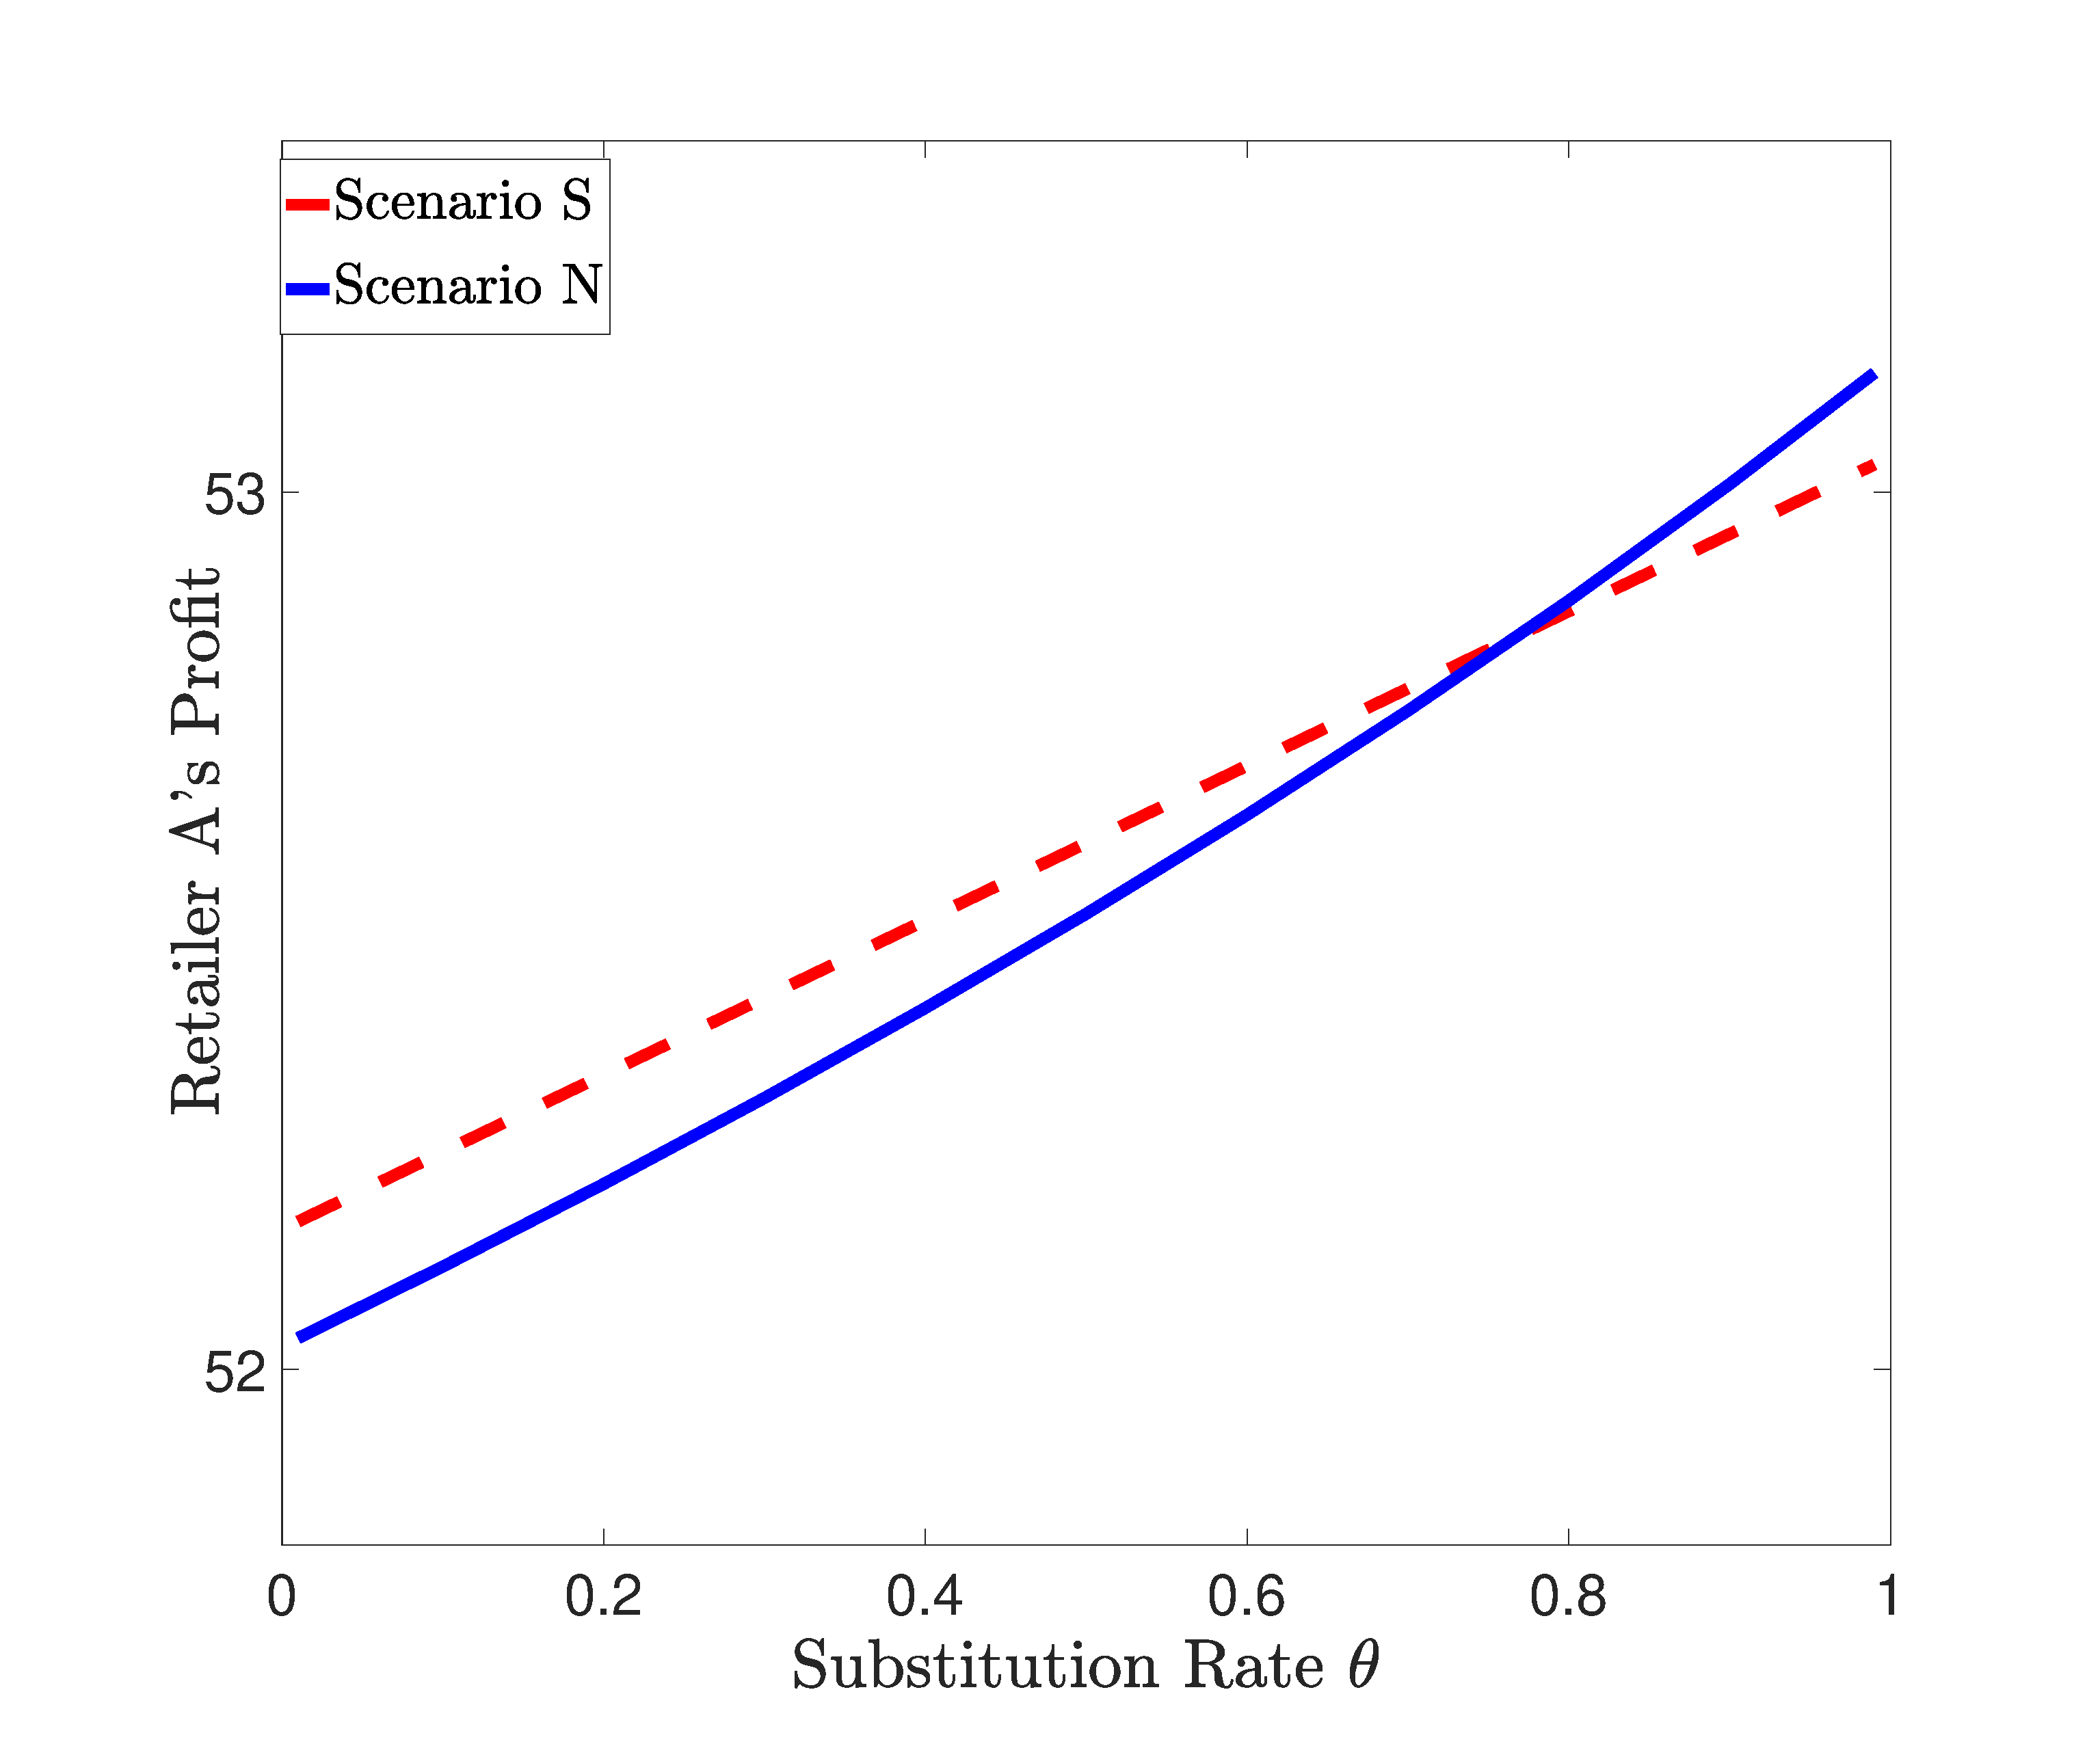
\includegraphics[width=\linewidth]{figure1.eps}
  \caption{Retailer A comparison; $\gamma = 0.7$}
  \label{fig:comparepfta-1}
\end{subfigure}
\begin{subfigure}{.42\linewidth}
  \centering
  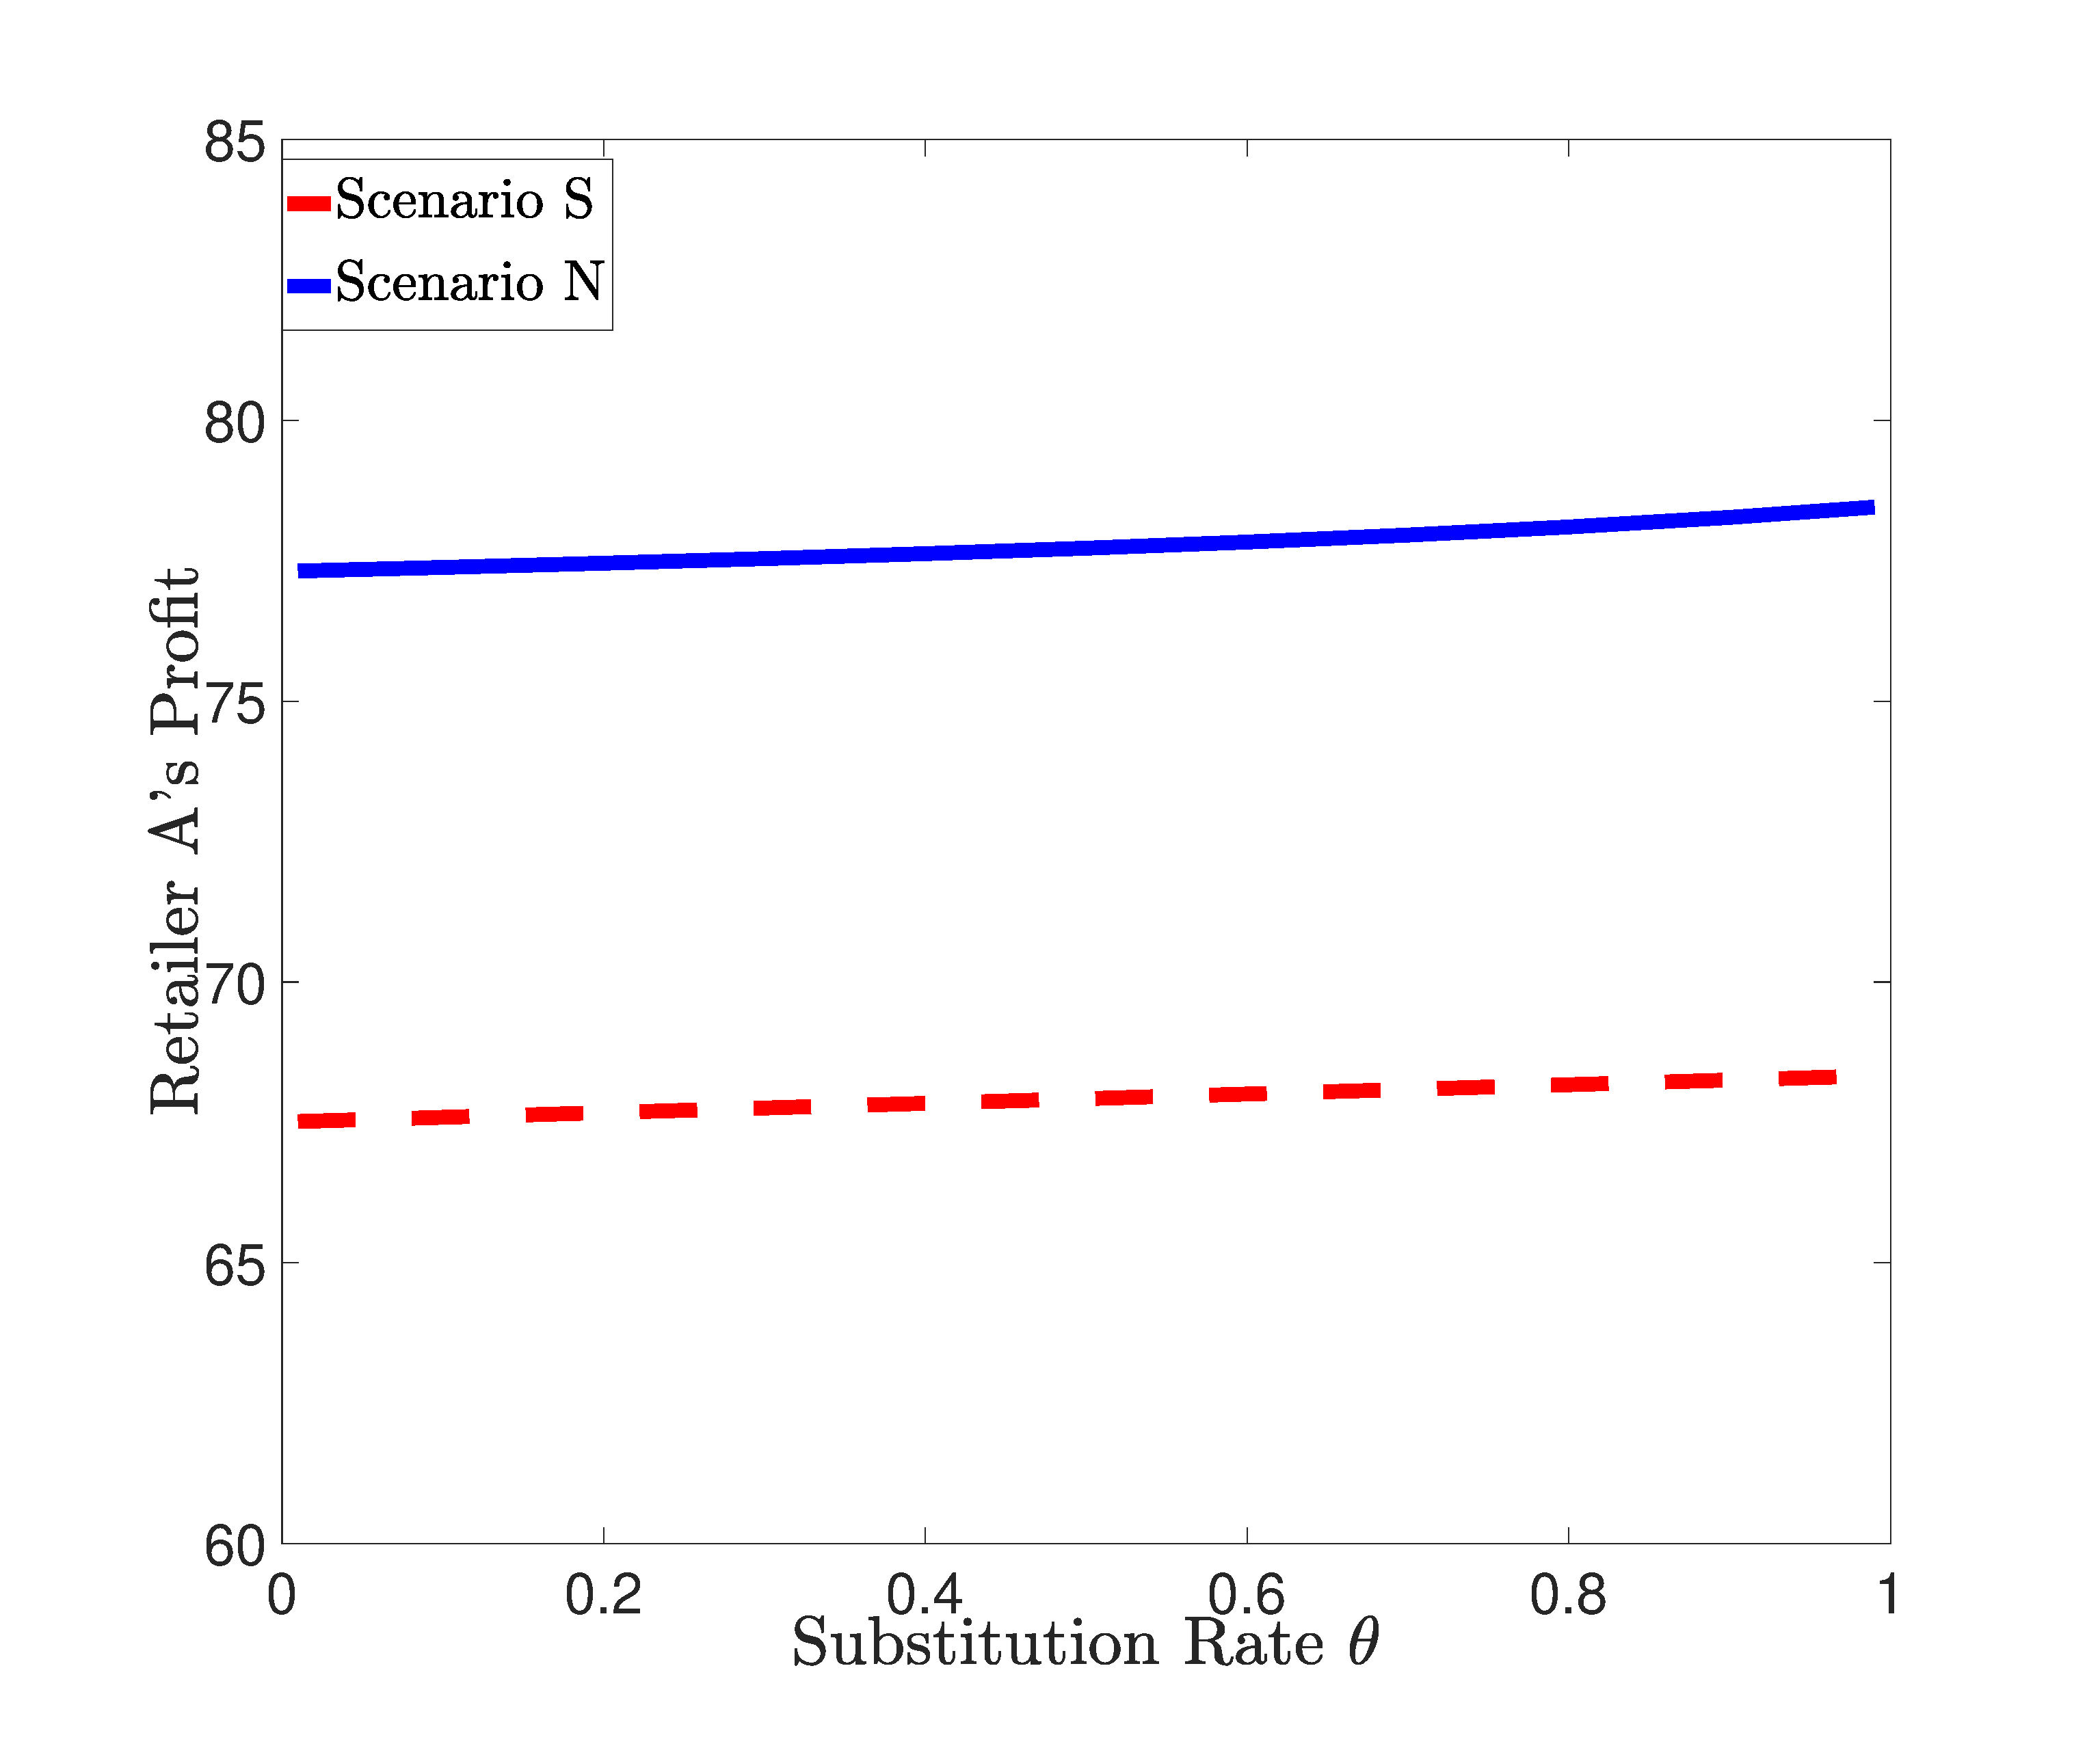
\includegraphics[width=\linewidth]{figure2.eps}
  \caption{Retailer A comparison; $\gamma = 2$}
  \label{fig:comparepfta-2}
\end{subfigure}
\\
\begin{subfigure}{.42\linewidth}
  \centering
  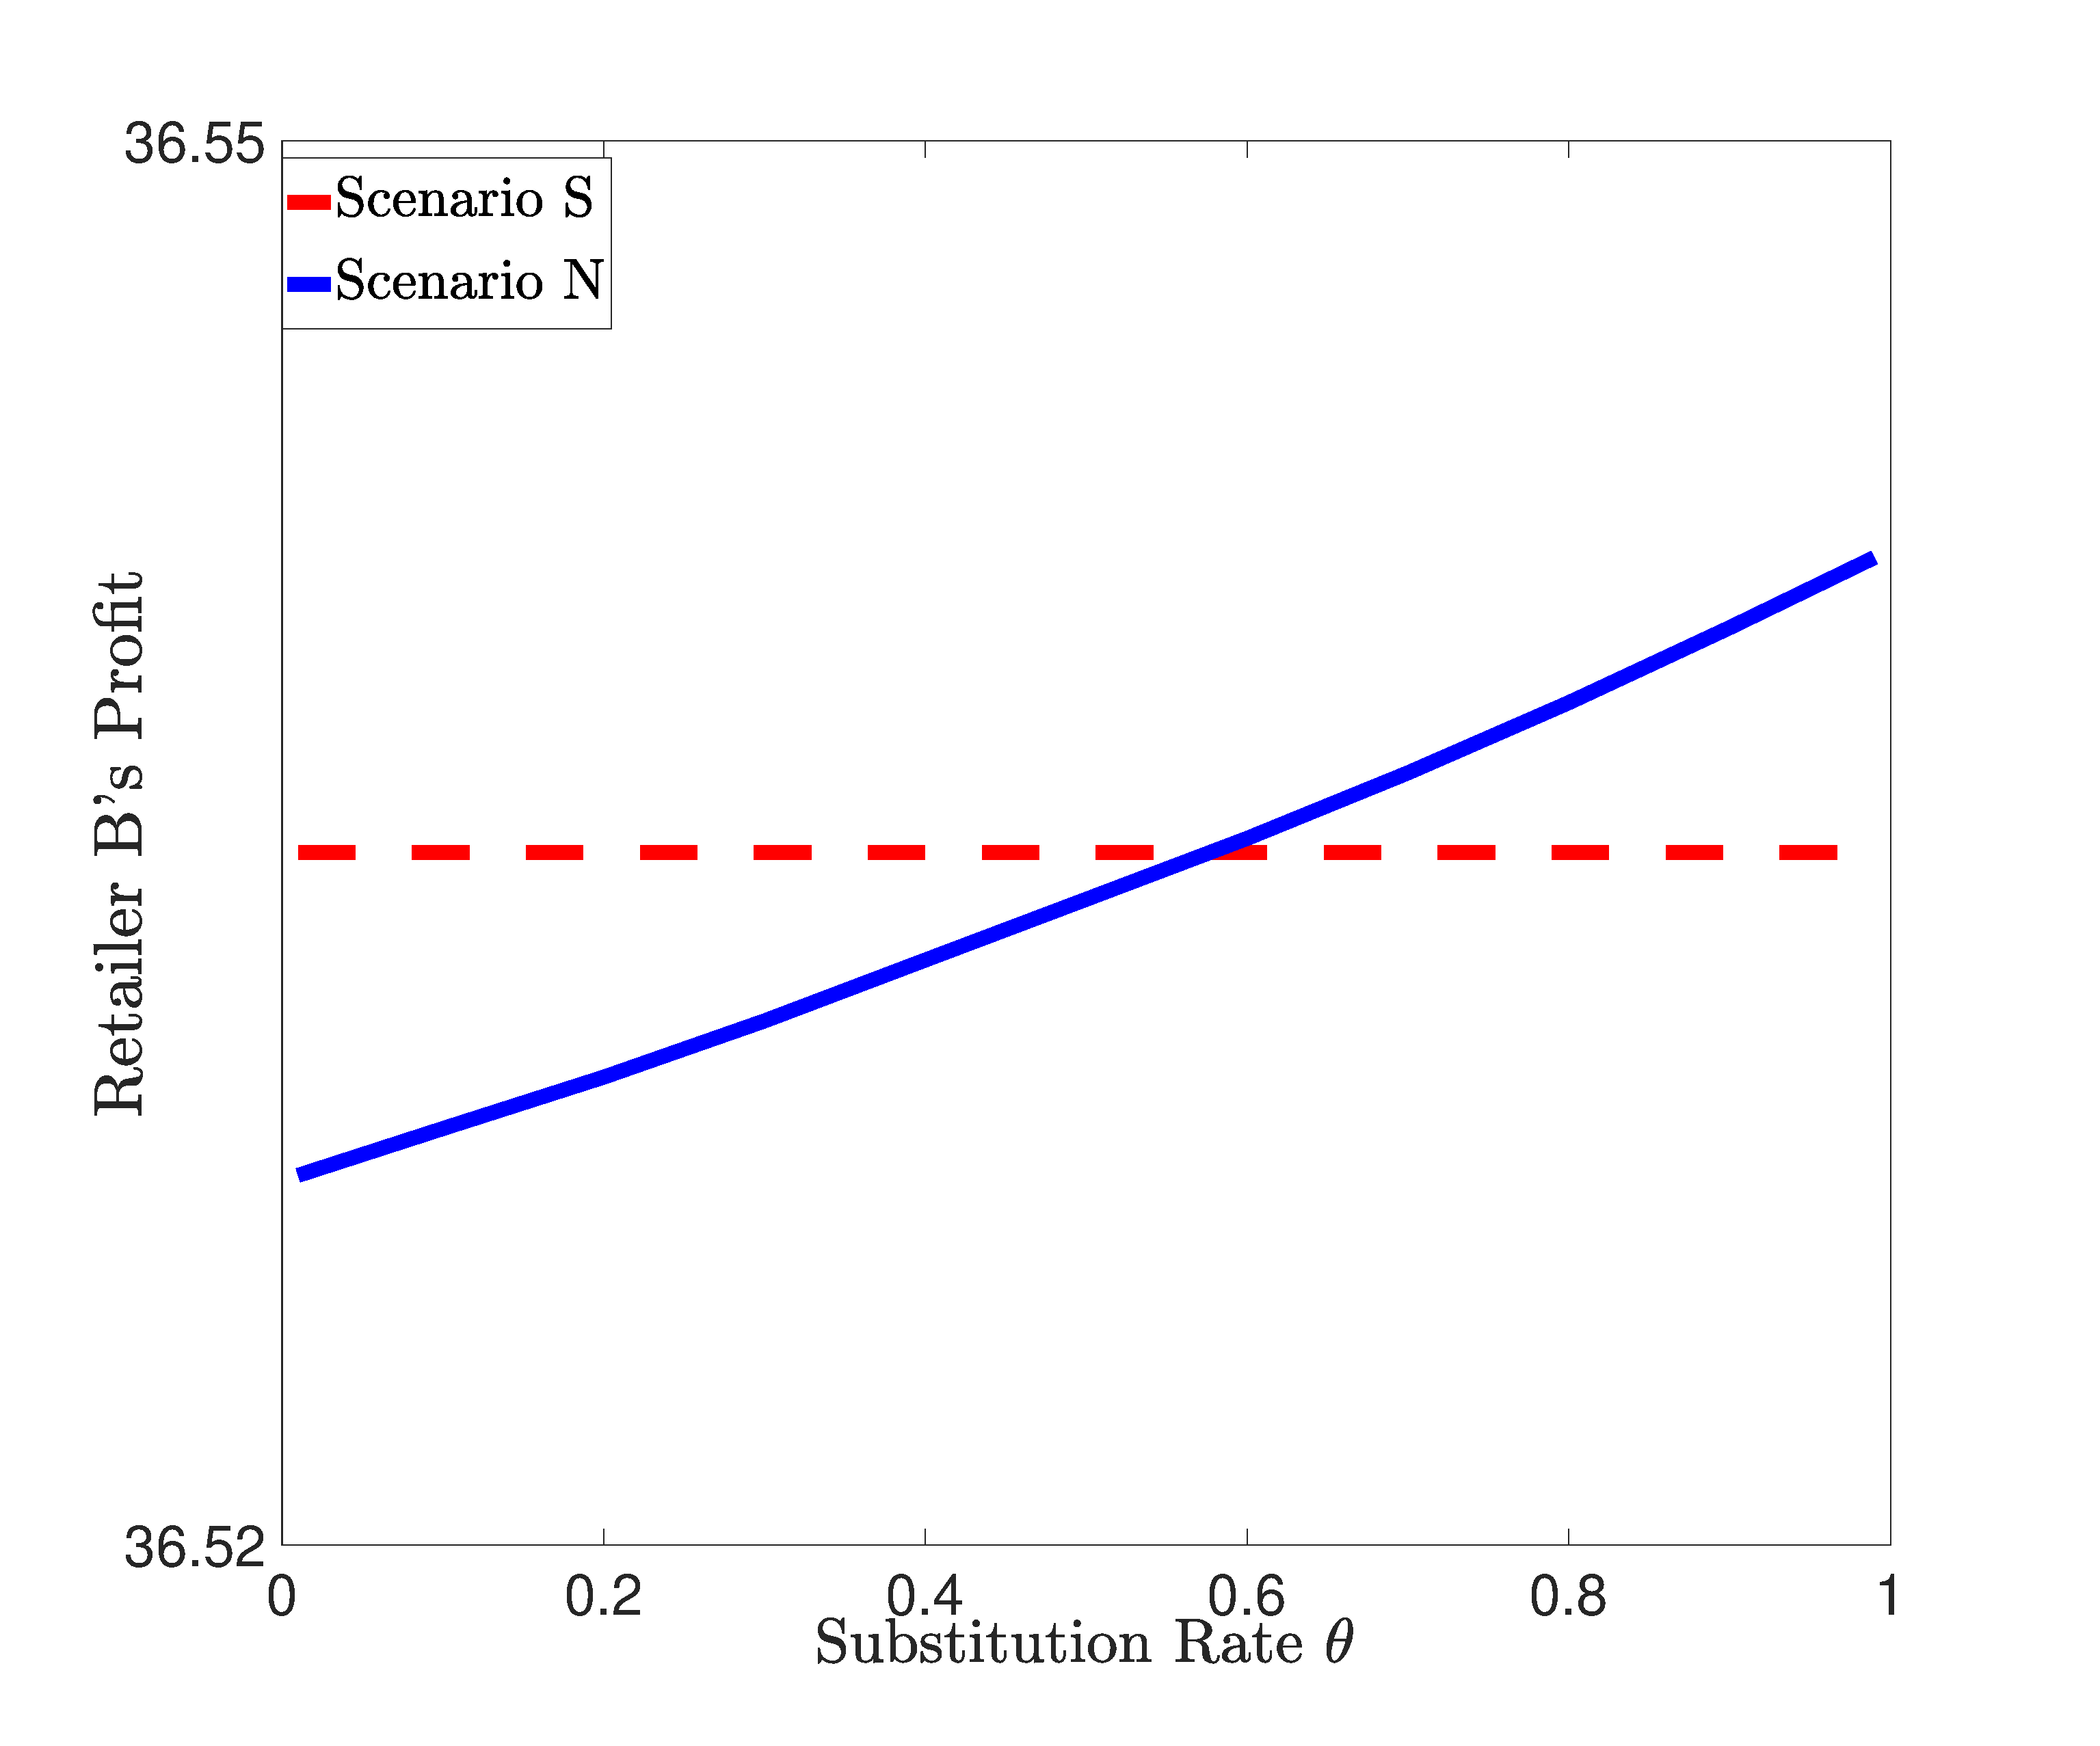
\includegraphics[width=\linewidth]{figure3.eps}
  \caption{Retailer B comparison; $\gamma = 0.7$}
  \label{fig:comparepftb-1}
\end{subfigure}
\begin{subfigure}{.42\linewidth}
  \centering
  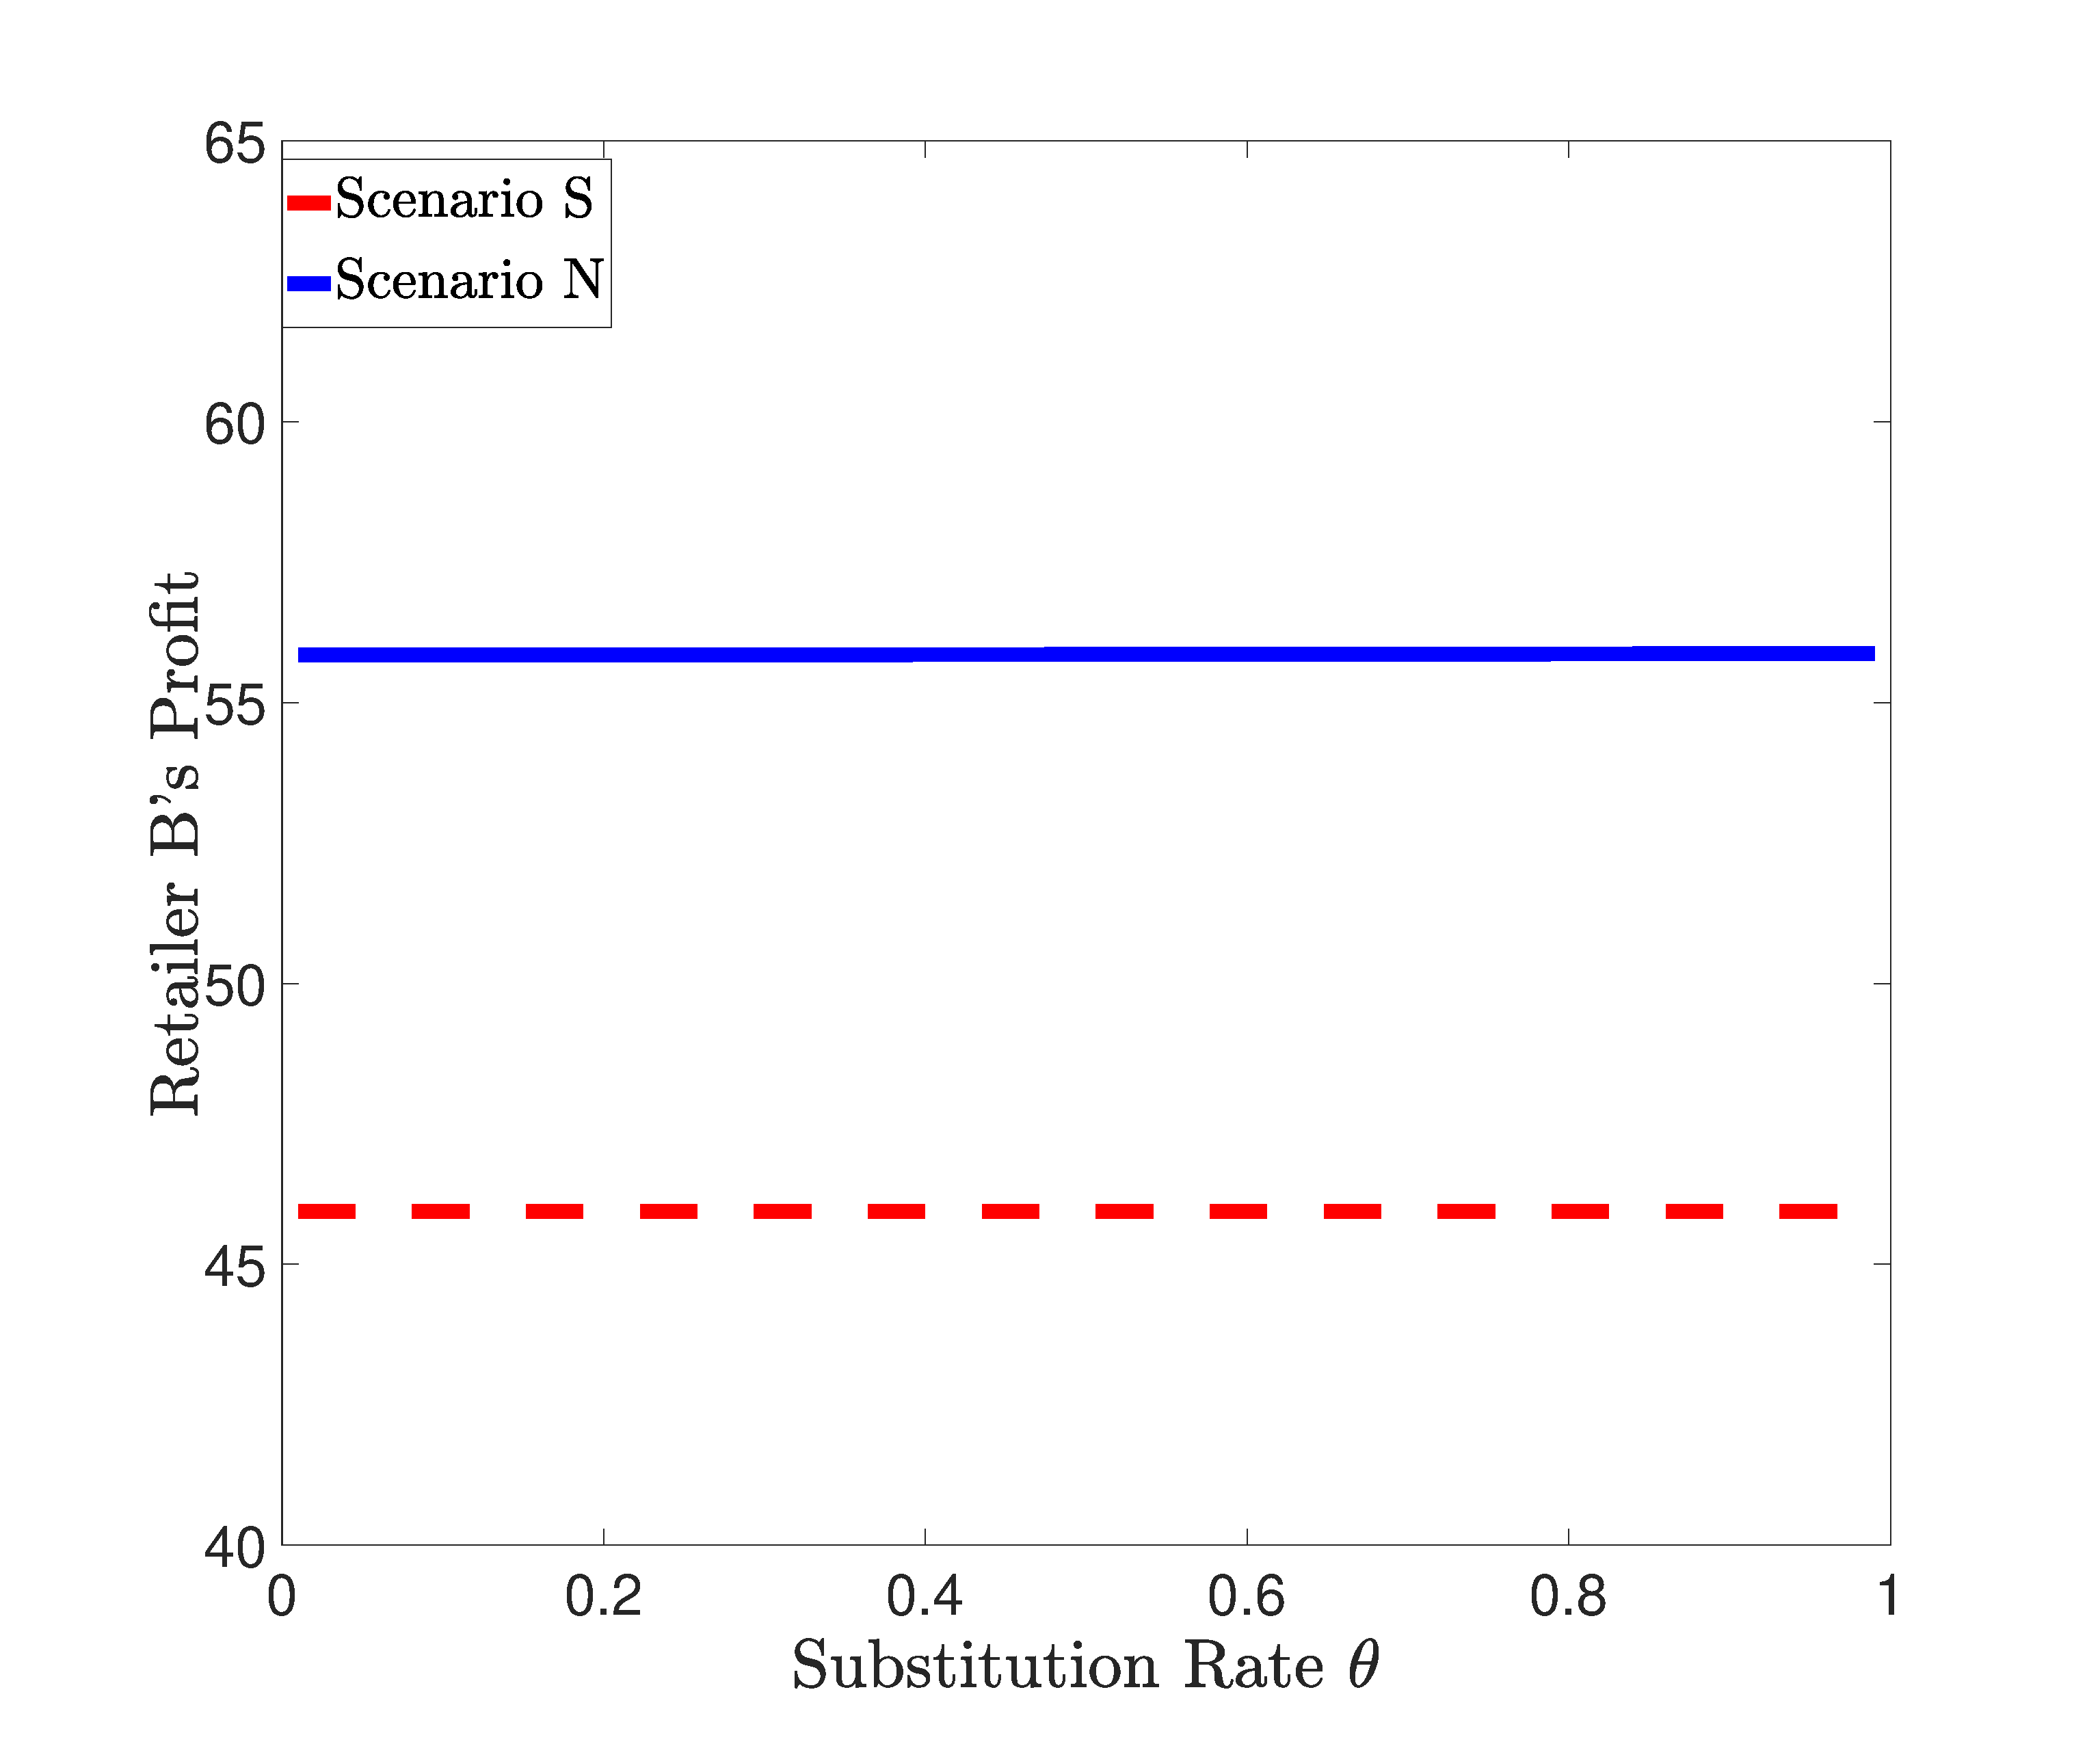
\includegraphics[width=\linewidth]{figure4.eps}
  \caption{Retailer B comparison; $\gamma = 2$}
  \label{fig:comparepftb-2}
\end{subfigure}

\begin{flushleft}
    {\footnotesize \emph{Parameters:} We pick $p_{i,t} \in \{2,4\} (i = A, B; t = 1, 2)$, and fix $c_B=1$, $\beta=0.1$, $X_t \sim U[5,15] (t = 1, 2)$. For retailer A's comparison, we choose $c_A = 0.1$; and for retailer B's comparison, we choose $c_A = 0.95$. }
\end{flushleft}
\end{figure}

From these graphs, we gather observations regarding the retailers' total profits under equilibrium pricing across different scenarios, with the strength of C2C interactions varying.
Before diving into the specific findings, we highlight an important distinction between the current analysis and that in Section~\ref{sec:compare}. Previously, both scenarios were evaluated under exogenously fixed retail prices, whereas here, prices are determined endogenously and may differ across scenarios. In general, when prices are continuous and constrained within a bounded interval, the equilibrium market split ratio between the two retailers may vary across periods. However, in our numerical experiments, although the equilibrium prices across the two periods may not be the same, the resulting split ratios remain constant over time. This feature simplifies the analysis and enables us to focus on the particularly insightful case, i.e., $\alpha_{i,1} = \alpha_{i,2}$ for $i = A, B$, where the retailers' profit functions in the two scenarios are directly comparable and may intersect.

With this in mind, we summarize two key observations from the numerical results. First, Figure \ref{fig:compare}(a)\&(c) replicate the results in Propositions \ref{prop:pfta}\&\ref{prop:pftb} under a moderate $\gamma$. For retailer A, as $\theta$ increases to 1, Scenario N becomes more profitable than Scenario S. For retailer B, when $\theta$ is small, Scenario S yields higher profit. These outcomes align with our earlier findings, as the parameter choices reflect the required conditions, namely, a non-negligible level of social interactions and a large [resp., small] cost difference for retailer A’s [resp., B’s] comparison. Moreover, although we restrict the feasible price set to two discrete values in the numerical experiments, this setup preserves the core mechanism of endogenous pricing and allows meaningful equilibrium comparisons.

Second, Figures \ref{fig:compare}(b)\&(d) illustrate how the earlier theoretical results may not hold when C2C interactions become very strong in the Endogenous Price Model. Specifically, Figure \ref{fig:compare}(b) shows that retailer A always earns more in Scenario N, even when $\theta$ is small and $\alpha_{A,1} = \alpha_{A,2}$ --- an outcome not seen before. This can be explained by the intensified price competition in Scenario S under large $\gamma$, which suppresses retailer A's first-period profit. Figure \ref{fig:compare}(d) further shows that, across all $\theta$ values, retailer B consistently earns more in Scenario N, even though $\alpha_{B,1} = \alpha_{B,2}$. In fact, in Scenario S, although retailer B can expand its own market share, it cannot do it effectively due to retailer A’s advantageous cost-efficiency and the resulting pricing dominance.

Taken together, these results suggest that when retailers engage in endogenous pricing, strong social interactions can fundamentally alter the profit comparison. In such cases, the crossover pattern predicted in Propositions \ref{prop:pfta}\&\ref{prop:pftb} may no longer appear, and one scenario may dominate the other for the entire range of $\theta$. Thus, to extend the previous propositions to this endogenous pricing setting, one might need to impose an upper bound on $\gamma$. Intuitively, this is because pricing flexibility enables retailers to make aggressive markdowns that help capture more market share while amplifying the benefit from strong social interactions.

\section{Concluding Remarks}\label{sec:con}

Online retailing has grown increasingly dynamic and competitive, with customer behavior shaped not only by product availability and price but also by the social interactions embedded in the shopping experience. This is particularly salient in formats like live video shopping, where past sales and customer engagement can generate C2C-induced demand. In this paper, we take a novel approach to study two types of C2C interactions that generate different forms of demand growth. Under within-brand interactions (Scenario S), realized sales generate C2C-induced demand attributed to the originating retailer. In contrast, under cross-brand interactions (Scenario N), both retailers’ realized sales contribute to an incremental common market that can subsequently be captured by either retailer. These two mechanisms govern the market growth over time and induce very different competitive dynamics.
To investigate these effects, we develop a two-period duopoly model in which newsvendor-type retailers with asymmetric costs compete in inventory and price. Below, we summarize the main findings and managerial implications.

First, under cross-brand C2C, the high-cost retailer (retailer B) may benefit from the market expansion driven by the low-cost retailer's (retailer A's) sales. In this case, retailer B strategically orders less and allows excess demand to spill over to retailer A, who carries more inventory at lower cost. Retailer B then reaps the rewards of the expanded market in the second period, without incurring much cost itself. This behavior demonstrates the possibility of demand ``free-riding'' through social interactions and suggests that a high-cost online retailer, when facing a more efficient competitor, can capitalize on its rival's operational advantage to gain market access through cross-brand social contagions. Meanwhile, the inventory decisions of retailer A are shaped by the nature of the C2C interaction, with the intensity of inventory competition playing a central role in determining its strategic response.

Second, the comparison of retailers' total profits under different types of C2C interactions reveals an interesting finding regarding their scenario preferences. While it may seem intuitive that the low-cost [high-cost] retailer benefits more under within-brand [cross-brand] interactions, our results show this intuition does not always hold. When the low-cost retailer has already secured a strong competitive edge, the added intensity from within-brand interactions may hurt rather than help, making cross-brand interactions more profitable. Conversely, if the high-cost retailer is not too disadvantaged, it can perform better under within-brand interactions, which contribute to a more competitive environment. These findings suggest that both competitive and collaborative forces shape the equilibrium outcomes, and online retailers may benefit most from a balanced interplay between the two.

Third, when prices are endogenously determined, the equilibrium price paths differ sharply across scenarios. Under within-brand C2C, retailers set lower first-period prices to build realized sales and the associated seller-specific C2C-induced demand, and then raise prices to capitalize on this demand advantage. Under cross-brand C2C, prices decline over time as retailers compete more aggressively in the second period to capture a larger share of the expanded common market. Our earlier profit-comparison patterns largely persist under endogenous pricing, although sufficiently strong C2C interactions may alter them. These results underscore how different types of C2C-induced demand shape the interaction between pricing and inventory decisions.

To conclude, our aggregate demand dynamics are modeled in reduced form and are not derived from a formal consumer-level micro-foundation. Although existing research separately supports the component mechanisms, it does not jointly derive C2C-induced demand formation, customer choice, product availability, post-stockout search, and substitution within a single structural model. Further research is therefore needed to develop an integrated consumer-level framework that incorporates these model elements. In addition, we point out several interesting avenues for future studies that could extend this paper in multiple directions.
(1) In practice, the strength of C2C interactions may fluctuate due to varying customer engagement levels. Incorporating stochastic interaction strength would allow us to study how uncertainty in C2C-induced demand affects retailers' strategic decisions and competitive dynamics.
(2) If the retailers sell nonperishable products, inventory may carry over across periods. This would introduce richer system dynamics, where inventory positions evolve over time and the equilibrium order quantities become more intricate.
(3) From a supply chain management perspective, the model can be extended to incorporate upstream manufacturers. C2C-induced demand may then have cascading effects across the supply chain, prompting new forms of strategic response from different channel members.

\begin{flushleft}
\bibliographystyle{ormsv080}
\bibliography{reference2024}
\end{flushleft}

\end{document}
